\documentclass[a4paper, 12pt]{article}
\usepackage{outlines}
\usepackage{graphicx}
%\usepackage{times}
\usepackage{xcolor}
\usepackage{float}
\usepackage{mathtools}
\usepackage{enumerate}
\usepackage{geometry}
\usepackage[english]{babel}
\usepackage{array}
\usepackage{wrapfig}
\usepackage{amsmath}
\usepackage{multirow}
\usepackage{tabu}
\usepackage{titlesec}
\usepackage{titletoc}
\usepackage{array}
\usepackage{tabularx,ragged2e,booktabs,caption}
\usepackage{chngcntr}
\usepackage{pgf-pie}  
\counterwithin{figure}{section}
\counterwithin{table}{section}
\usepackage{colortbl}

\titleformat{\section}[display]%
{\null\fontsize{16}{5}\rmfamily\bfseries\filcenter}{CAPITOLUL \thesection}{1em}{}[]
\titleformat{name = \section, numberless}[block]%
{\null\fontsize{16}{5}\rmfamily\bfseries\filcenter}{}{1em}{}
\titlespacing*{\section}{0em}{1em}{1em}

\titlecontents{section}
[7em] % ie, width of contentslabel + 0.5em
{\medskip}
{\contentslabel[\MakeUppercase\chaptername~\thecontentslabel]{7.5em}}%\thecontentslabel
{\hspace*{-6.5em}}
{\titlerule*[0.5pc]{.}\contentspage}

\addto{\captionsenglish}{
	\renewcommand{\refname}{Referințe bibliografice}%
	\renewcommand{\contentsname}{Cuprins}
	\renewcommand{\listfigurename}{Lista imaginilor}
	\renewcommand{\listtablename}{Lista tabelelor}
}
\addto\captionsenglish{\renewcommand{\chaptername}{Capitolul}}
%define the page geometry
\geometry{
	a4paper,
	left=25mm,
	top=25mm,
	bottom=25mm,
	right=25mm,
}
\renewcommand{\baselinestretch}{1.5}
\makeatletter
\renewcommand\paragraph{\@startsection{paragraph}{4}{\z@}%
	{-2.5ex\@plus -1ex \@minus -.25ex}%
	{1.25ex \@plus .25ex}%
	{\normalfont\normalsize\bfseries}}
\makeatother
\setcounter{secnumdepth}{4} % how many sectioning levels to assign numbers to
\setcounter{tocdepth}{4}    % how many sectioning levels to show in ToC



\begin{document}

%define the title page
\begin{titlepage}
	\begin{center}
		\vspace{0.5cm}
		\large {UNIVERSITATEA "BABEȘ-BOLYAI" CLUJ-NAPOCA}
		
		\large {FACULTATEA DE STUDII EUROPENE}
		\\
		
		
		\vspace{6cm}
		
		\Huge \textbf{LUCRARE DE LICENȚĂ}
		
		\vspace{2 cm}
		
		\vfill
	\end{center}
	
	\begin{flushleft}
		\large{\textit{Coordonator științific:}} \\
		\large{Conf. univ. dr. Nicoleta Dorina Racolța-Paina}
	\end{flushleft}
	
	\begin{flushright}
		\hfill \large {\textit{Absolvent:}} \\
		\hfill \large {Sorina-Elena Ciucanu}
	\end{flushright}
	
	\begin{center}
		\vspace{1.5cm}
		\large \textbf{2021}
	\end{center}
\end{titlepage}
\begin{titlepage}
	\begin{center}
		\vspace{0.5cm}
		\large {UNIVERSITATEA "BABEȘ-BOLYAI" CLUJ-NAPOCA}
		\\
		\large {FACULTATEA DE STUDII EUROPENE}
		\\\large {SPECIALIZAREA MANAGEMENT}
		
		\vspace{2.75cm}
		
	
		\huge Comportamentul consumatorului online, tânăr și educat din România
		
		\huge Studiu de caz
		\vspace{1.5 cm}
		
		\vfill
	\end{center}
	
	\begin{flushleft}
		\large{\textit{Coordonator științific:}} \\
		\large{Conf. univ. dr. Nicoleta Dorina Racolța-Paina}
	\end{flushleft}
	
	\begin{flushright}
		\hfill \large {\textit{Absolvent:}} \\
		\hfill \large {Sorina-Elena Ciucanu}
	\end{flushright}
	
	\begin{center}
		\vspace{1.5cm}
		\Large{Cluj Napoca}
		
		\large \textbf{2021}
	\end{center}
\end{titlepage}
\restoregeometry
\thispagestyle{empty}
\section*{Declarație}
\bigskip
\qquad Prin prezenta declar că Lucrarea de licenţă cu titlul "Comportamentul consumatorului online tanar si educat din Romania. Studiu de caz" este scrisă de mine şi nu a mai fost prezentată niciodată la o altă facultate sau instituţie de învăţământ superior din ţară sau străinătate. De asemenea, declar că toate sursele utilizate, inclusive cele de pe Internet, sunt indicate în lucrare, cu respectarea regulilor de evitare a plagiatului:
\begin{enumerate}[-]
	\item toate fragmentele de text reproduse exact, chiar şi în traducere proprie din altă limbă, sunt scrise între ghilimele şi deţin referinţa precisă a sursei;
	\item reformularea în cuvinte proprii a textelor scrise de către alţi autori deţine referinţa precisă;
	\item rezumarea ideilor altor autori deţine referinţa precisă la textul original.
\end{enumerate}

\vspace{3 cm}
\begin{flushleft}
	\large Cluj Napoca,
\end{flushleft}


\begin{flushright}
	\hfill \large Absolvent \textit{Sorina-Elena Ciucanu} \\
	\hfill \large {(semnătura olograf)}
\end{flushright}
\newpage
\thispagestyle{empty}
%put the table of contents
\tableofcontents
\thispagestyle{empty}
%put the list of figures
\newpage
\thispagestyle{empty}
\listoffigures
\newpage
\thispagestyle{empty}
\listoftables

%this section is on new page
\newpage
%\nocite{bobalcua2015loyal}
%\nocite{london_economics_2011}
%\nocite{duralia2016particularities}
%\nocite{devderea2018consumer}
%\nocite{armstrong2014principles}
%\nocite{orzan2014study}
%\nocite{obradattitudes}
%\nocite{sava_2020}
%\nocite{bighiu2015compulsive}
%\nocite{gorunescu_2020}
%\nocite{orangehelp}
%\nocite{wall_2019}
%\nocite{ruxandra_andrei_2020}
%\nocite{sandulescusandulescu2020}
%\nocite{anastasiei_dospinescu_2019}
%\nocite{dobre2015personality}
%\nocite{dumitrescu2015understanding}
%\nocite{cetinua2018modelling}
%\nocite{babin_harris_2016}
%\nocite{usda foreign agricultural service_2021}
%\nocite{mihaela2019business}
%\nocite{csandor2013metode}
%\nocite{fuciu2019usage}
%\nocite{onete2016analysis}



 
	\section*{Introducere}
\addcontentsline{toc}{section}{\textsc{Introducere}}
	
	\quad\quad Lucrarea de față, "Comportamentul consumatorului online român, tânăr și educat- Studiu de caz" abordează un subiect vast și de actualitate, care devine din ce în ce mai important pentru firmele care doresc să-și dezvolte strategii de marketing axate pe factorii ce determină consumatorul online să aleagă un producător în detrimentul altuia. Numărul de studii publice pe tema procesului de cumpărare a consumatorului online din România este mic comparativ cu numărul de articole din alte țări, atât din Uniunea Europeană cât și din afară acesteia. Dorim să precizăm că această lucrare pune accentul pe consumatorul  individual și nu pe cel organizațional (entități juridice) deoarece dorim să analizăm ce anume determină cumpărătorul individual să achiziționeze produse care sunt de larg consum.
	
	\quad Scopul prezentei lucrări de licență este realizarea unui profil al consumatorului online tânăr și educat din România pentru ca firmele din comerțul electronic să înțeleagă mai bine comportamentul acestuia și să se plieze pe nevoile și dorințele lui.
	
	\quad Prezentul studiu își propune să prezinte principalele aspecte teoretice cu privire la comportamentul consumatorilor online, respectiv practice referitoare la factorii care influențează comportamentul consumatorului online român,tânăr și educat, pentru ca în final să oferim informații de folos companiilor ce practică comerțul electronic și sunt prezente pe piața din România.
	
	\quad La fel ca orice demers științific, este nevoie de existența unei baze teoretice care să vină în ajutorul analizei informațiilor obținute în urma studiului de caz. Astfel, pentru partea teoretică este utilizată cartea fondatorului marketing-ului, Philip Koetler, articole de la Comisia Europeană, privind la nivel de Uniune consumatorul online, dar și câteva articole de la autori români precum Duralia Oana de la Universitatea Lucian Blaga din Sibiu și Claudia Bobâlcă care și-au manifestat interesul față de percepția consumatorilor online, tineri asupra bunurilor online. 
	
	\quad Partea practică reprezintă o cercetare primară cantitativă, metoda folosită fiind sondajul de opinie, iar instrumentul de culegere a datelor fiind chestionarul (lansat online în perioada 27.04.-04.05) . Chestionarul folosit (vezi Anexa 1) cuprinde 3 întrebări filtru și anume una legată de vârstă( intervalul țintit de noi fiind 18-30 ani), o altă întrebare legată de nivelul de studii (minim BAC) și respectiv numărul de achiziții online, cu plata card în februarie-aprilie 2021 (aici dorind să avem răspunsuri de la consumatorii avizați). Am ales că respondenții să aibă un anumit interval de vârstă și anume 18-30 deoarece în domeniul marketing-ului este necesară poziționarea și segmentarea pieței țintă.
	
	\quad Structura lucrării include atât o secțiune teoretică cât și o secțiune practică, având în total un număr de 3 capitole. Primul capitol, numit "Comportamentul consumatorului online - conținut și tendințe" cuprinde 6 subcapitole, în care se discuta la modul general despre consumatorul online. Astfel, prima parte a capitolului cuprinde o introducere  comerțului electronic și anumite bariere ce se regăsesc în mediul digital. Pe urmă, lucrarea pune accent pe consumatorul online începând cu importanța comportamentului consumatorului,  managementul relațiilor cu clienții - metodă folosită astăzi de companii pentru a-și loializa clienții, tipuri de decizii pe care consumatorii obișnuiesc să le facă, apoi cu  modele de marketing care fac legătură dintre tehnologie și consumatorul online. Capitolul continuă cu identificarea generațiilor de consumatori si trend-urile prezente în cererea cumpărătorilor , apoi urmând factorii care tind să influențeze decizia de cumpărare a acestuia, procesul de cumpărare împărțit și detaliat pe etape. Ultimele doua subcapitole se referă la  beneficiile și provocările, pe care consumatorii online le-au întâlnit și depășit în experiențele lor în mediul online, iar în încheiere, am realizat o scurtă comparație între ecommerce și marketplace.
	
	\quad Al doilea capitol, numit "Cercetare secundară privind comportamentul constumatorului online, tânăr și educat din România" cuprinde 4 subcapitole. Primul subcapitol relevă informații despre comerțul electronic din România oferind statistici despre cumpărăturile online ale românilor, categoriile de produse care sunt achiziționate cel mai frecvent, online, de populația din România și contextul actual al pandemiei Covid19 care a avut o influență puternică asupra achizițiilor online. Următoarele subcapitole includ trei perspective asupra achizițiilor online din România, articole ce oferă informații despre comportamentul consumatorului online, tânăr și educat din România, iar la final o scurtă concluzie a celor trei articole.
	
	\quad Lucrarea continuă cu al treilea capitol, care cuprinde cercetarea propriu-zisă și reprezintă esența prezenței lucrări științifice deoarece realizează conexiunea între elementele teoretice cuprinse în capitolele anterioare și modul în care se aplică acestea în practică. Astfel, după cum am menționat anterior, în elaborarea acestui capitol este utilizat o metodă de cercetare cantitativă (instrumentul folosit fiind chestionarul) pentru a obține informațiile necesare atingerii obiectivelor propuse și anume, crearea unui profil al consumatorului online, tânăr și educat din România.
	
	\quad Lucrarea prezintă o serie de limite ca urmare a lipsei surselor bibliografice și studiilor datorat numărului scăzut de cercetări asupra comportamentului consumatorului online, tânăr și educat din România. De asemenea, reticiența respondenților de a răspunde la chestionar, în special a respondenților de genul masculin, mi-a îngreunat munca în cercetarea mea cantitativă. Un aspect neașteptat a fost numărul mare de respondenți care au ales la întrebarea filtru, referitoare la numărul minim de achiziții online în perioada februarie-aprilie 2021, mai puțin de 5 achiziții online, fapt ce m-a determinat să nu includ în cercetarea mea o mare parte din totalul de respondenți.
	
	\quad Luând în considerare cele afirmate mai sus, exprimăm speranța că această cercetare aduce un plus de valoare pentru domeniul teoretic, referitor la comportamentul consumatorului online, tânăr și educat din România și implicarea sa în comerțul electronic.
		
	\newpage
	\setcounter{section}{0}
	\section{Comportamentul consumatorului online - conținut și tendințe}
	
	\quad\quad Societatea în care trăim se află într-o continuă stare de schimbare. Ultimii ani de evoluție în domeniul comunicației, tehnologiei, informației și marketingului au creat noi schimbări în modul în care consumatorii se informează și cumpără anumite produse și servicii. În acest capitol se discută despre nouă modalitate, folosită în marketing, pentru a facilita schimbul de produse dintre cumpărător și producător, prin intermediul internetului, și anume, comerțul electronic. Apoi, se analizează comportamentul consumatorului fizic și online prin prisma a mai multor concepte și procese ce ne ajută să înțelegem gândirea și comportamentului acestuia. 

		\subsection{Comerțul electronic}
	\quad \quad\space În ultimii zece ani, în contextul internațional al comunicării digitale, comerțul electronic devine o importantă parte a sistemului de afaceri. Odată ce Internetul a devenit un instrument foarte utilizat și important în comunicare, promovare și tranzacții comerciale, noi platforme s-au dezvoltat pentru a crea strategii competitive.
	
	\quad Diverse articole susțin faptul că comercializarea produselor este încă necesară și vitală, însă nu mai este suficientă pentru ca o companie să-și păstreze poziția pe piață. Astfel s-a introdus un nou concept numit experiența clienților, definit drept "răspunsul intern și subiectiv pe care îl au clienții la orice contact cu o companie", pentru a descrie noua relație dintre brand-uri și clienți.\footnote{Mihaela Știr, "Business to consumer- Ecommerce in România-Evolution and trends", 2019, p.128} Noile așteptări ale consumatorilor moderni sunt influențate de schimbările tehnologice care au afectat structurile comerciale, crescând interesul consumatorilor pentru E-commerce. Că să putem fi mai clari, vom defini comerțul electronic drept "orice formă de tranzacție comercială unde părțile implicate interacționeaza într-un mod electronic".\footnote{Claudia Bobalca, \textit{"The Loyal Customers’ Perception Regarding The Online Buying Process"}, Economie, p.241}	
	
	\quad Într-o economie globală, dezvoltată într-o piață foarte competitivă, orientarea spre consumator nu mai reprezintă doar un trend ci o necesitate, precum am menționat și anterior. Astfel, o bună înțelegere a modului în care consumatorii beneficiază de proprietățile Internetului și a factorilor pe care îi iau în considerare pentru a se hotărâ asupra deciziilor de cumpărare în mediul comerțului electronic, aduce avantaje semnificative pentru managerii care doresc să dezvolte strategii de marketing potrivite profilului consumatorilor pe care îi au. Cumpărătorii online au acces nelimitat la informație și au oportunitatea de a alege dintr-o gama largă de opțiuni în selectarea produselor și serviciilor potrivite acestora.\footnote{Radu Lixandroiu, Ana-Maria Cazan, Catalin Ioan Maican, 2019, \textit{An Analysis of the Impact of Personality Traits towards
			Augmented Reality in Online Shopping}, p.1-2}

	\quad În acest caz, merită remarcat faptul că ecommerce-ul include ambele tipuri de tranzacții implicând atât bunuri tangibile precum electronice, bunuri de larg consum, jucării care trebuie să fie livrate fizic către consumator, dar și tranzacții privind accesul la bunuri intangibile, precum sevicii sau produse care pot fi furnizate digital către consumator. De asemenea, trebuie menționat faptul că există bunuri care se găsesc atât în format electronic cât și în format fizic precum cărțile, revistele, muzică și jocurile.

	\quad În urma experiențelor privind achiziția unor produse/servicii online, unii consumatori au întâlnit și câteva bariere care i-a determinat să evite mediul digital, printre care principalele le enumerăm mai jos\footnote{European Parliament, D.G.I.P. 2011. \textit{Consumer Behaviour in a Digital Environment}. Brussels.}:
	\begin{itemize}
	\item Potrivit rezultatelor de la Eurostat cel mai frecvent motiv, pe care consumatorii l-au menționat, a fost preferința pentru cumpărături în format fizic sau faptul că nu simt nevoia de a utiliza mediul online pentru a plasa comenzi.
	\item Un alt motiv foarte des întâlnit, pe care îl menționează tot informațiile prezente de la Eurostat, sunt riscurile privind securitatea, intimitatea și grijile privind încrederea în a-și împărtăși datele personale pe care consumatorii le întâmpină atunci când doresc să plaseze o comandă online.
	\item De asemenea, consumatorii au adăugat că lipsa sau insuficiența informațiilor despre un anumit produs i-a determinat să evite achizițiile unor bunuri online.	
	\end{itemize}
\newpage
		\subsection{Comportamentul consumatorului}	
		\quad Acceptarea de către consumator, a internetului, drept un mijloc de informare, comparare de informații  și cumpărare a diverse bunuri și servicii a rezultat în ceea ce literatură de specialitate definește prin conceptul de e-consumator sau consumator electronic.\footnote{Oana Duralia. 2016. \textit{Particularities of the european consumer`s behaviour în online environments}, p.21}.  Spre deosebire de consumatorii tradiționali, care sunt mai conservatori și mai constanți în alegerile lor, e-consumatorii manifestă o deschidere mai mare pentru schimbare, fiind mult mai disponibili să încerce lucruri noi.\footnote{Ibidem} În plus, dacă ar fi să creăm un portret al e-consumatorului l-am putea descrie drept o persoană inovativă, creativă, educată, cu studii superioare și cu un status socio-economic ridicat.
			\subsubsection{Importanța comportamentului consumatorului }
		\qquad\space Precum am menționat și anterior, orientarea spre consumator și cunoașterea acestuia reprezintă un element cheie al companiilor ce vor să-și crească vânzările și să-și loializeze clienții. Astfel, este importantă identificarea și analiza comportamentului cumpărătorului pentru a obține succesul pe piață..
		
		\quad În articole și cărți există diverse definiții pentru comportamentul consumatorului. Conform Asociației de marketing din America comportamentul consumatorului este definit că: \textit{"interacțiunea dinamică a afectului și a cunoașterii, comportamentul și mediul prin care ființele umane desfășoară aspectele de schimb ale vieții lor"}. Alți autori definesc comportamentul consumatorului că fiind \textit{"studiul tuturor proceselor implicate în activitatea indivizilor sau grupurilor de indivizi care aleg, cumpără, utilizează sau elimină produsele, servicii sau idei care duc la satisfacerea nevoilor sau dorințelor consumatorilor"}. Specialiștii în marketing din România au convenit asupra unei definiții clare a conceptului de comportament al consumatorului că fiind: \textit{"toate actele decizionale ale individului sau ale grupului, legate direct de obținerea și utilizarea produselor și serviciilor, pentru a satisface nevoile prezente și viitoare, inclusiv toate procesele decizionale care preced și determină aceste acte"}.\footnote{Dumitrescu Luigi, Orzan Gheorghe, Fuciu Mircea. 2015. \textit{Understanding The Online Consumer Behaviour And The Usage Of The Internet As A Business Environment A Marketing Research}. Revista Economica. p.65} 
		
		\quad Din toate definițiile menționate mai sus și, de asemenea, din multe altele, putem vedea clar un model care apare în definirea comportamentului consumatorului. Acest model conține următoarele caracteristici:\footnote{Ibidem}

		\begin{itemize}
			\item Comportamentul consumatorului se referă la indivizi, precum și la grupuri sau
			organizații;
			\item Conține întotdeauna conceptul de a satisface o anumită nevoie sau dorință,
			vremea este una personală sau organizațională;
			\item Implică întotdeauna un anumit proces care duce la decizie;
		\end{itemize}
	
			\subsubsection{Managementul relațiilor cu clienții - CRM}
		\qquad Pe lângă orientarea spre consumator, care este importantă pentru menținerea avantajului competitiv și poziției pe o anumită piață, un alt element esențial îl reprezintă calitatea relației dintre un cumpărător și un producător, brand sau comerciant.
		
		\quad Acest lucru se numește, în teorie, \textbf{managementul relațiilor cu clienții - CRM}. Un astfel de sistem  urmărește informații detaliate despre clienți, astfel încât specialiștii de marketing să poată lua decizii orientate către clienți, care duc la relații mai durabile. Într-o orientare CRM, fiecare client reprezintă un flux potențial de resurse, mai degrabă decât o singură vânzare.\footnote{Babin J. Barry, Harris G. 2017. \textit{CB Consumer Behaviour}. Nelson Education. p.24-25} Astfel, conform definiției lui Koetler, am putea defini CRM drept "\textit{gestionarea informațiilor detaliate despre clienții individuali și gestionarea atentă a punctelor de contact ale clienților pentru a maximiza loialitatea clienților."}\footnote{Armstrong Gary, Adam Stewart, Denize Sara, Kotler Philip. 2012. \textit{Principles of martketing}. Pearson.p.12}
		
		\quad În practică, atunci când un consumator cumpără aceeași marca de fiecare dată când are o nevoie pentru acel produs, se creează o relație mult mai puternică deoarece întreprinderile văd clienții fideli că fiind mult mai profitabili decât clienții care sunt predispuși la schimbarea furnizorilor de fiecare dată când fac o achiziție.  
		
		\quad Prin utilizarea CRM pentru a înțelege mai bine clienții, companiile pot oferi un nivel mai ridicat de calitate pentru clienți și pot dezvoltă relații mai de lungă durată cu aceștia. De asemenea, ei pot folosi acest sistem pentru a identifica
		clienți de mare valoare, să le ofere o atenție sporită, și să creeze oferte adaptate cerințelor specifice ale clienților.
		
			\subsubsection{Tipuri de decizii}
				\qquad Comportamentul de cumpărare, fie el online sau fizic, diferă foarte mult în funcție de produsul pe care consumatorul vrea să-l achiziționeze. Astfel, deciziile mai complexe implică de obicei mai mulți participanți la cumpărare și mai mulți cumpărători prudenți. În viziunea lui Koetler, există patru mari tipuri de decizii pe care consumatorul le poate lua.\footnote{Armstrong Gary, Adam Stewart, Denize Sara, Kotler Philip. 2012. \textit{Principles of martketing}. Pearson. p.150}
			\begin{enumerate}[A)]
				\item \textbf{Comportamentul complex de cumpărare}
				
				\quad Acest tip de consumatori adoptă un comportament complex de cumpărare atunci când sunt foarte implicați într-o achiziție și percep diferențe semnificative între mărci. Consumatorii pot fi foarte implicați atunci când produsul este scump, riscant și achiziționat rar. De obicei, consumatorul are multe de învățat despre categoria de produse, însă uneori nu știe ce atribute să ia în considerare. Astfel acest cumpărător va trece printr-un proces de învățare, dezvoltând mai întâi credințe despre produs, atitudini și apoi făcând o alegere de cumpărare atentă. În acest caz, comercianțîi trebuie să îi ajute pe cumpărători să învețe despre atributele clasei de produse și despre importanța lor relativă.
				
				\item \textbf{Comportamentul de cumpărare prin reducerea dezacordului}
				
				\quad Comportamentul de cumpărare care diminuează dezacordul apare atunci când consumatorii sunt foarte implicați într-o achiziție costisitoare, mai puțîn frecventă sau riscantă, dar observă diferențe mici între mărci. De exemplu, consumatorii care cumpără covoare se pot confruntă cu o decizie de implicare ridicată, deoarece covoarele sunt scumpe. Cu toate acestea, cumpărătorii pot consideră că majoritatea mărcilor de covoare dintr-o anumită gamă de prețuri sunt aceleași. În acest caz, deoarece diferențele percepute de marcă nu sunt mari, cumpărătorii pot face cumpărături pentru a afla ce este disponibil, dar cumpără relativ repede. Acestea pot răspunde în primul rând la un preț bun sau la o comoditate de cumpărare.
				
				\quad După cumpărare, consumatorii ar putea experimenta dezacordul post-cumpărare (disconfort post-vânzare) atunci când observă anumite dezavantaje ale mărcii de covor achiziționate sau aud lucruri favorabile despre mărcile care nu au fost achiziționate. Pentru a contracara o astfel de disonanță, comunicările post-vânzare ale marketerului ar trebui să ofere dovezi și sprijin pentru a-i ajuta pe consumatori să se simtă bine cu privire la alegerile lor de marcă.
				
				\item \textbf{Comportamentul obișnuit de cumpărare}
				
				\quad Comportamentul obișnuit de cumpărare apare în condiții de implicare scăzută a consumatorilor și a unei diferențe semnificative de marcă. Consumatorii par să aibă o implicare redusă cu cele mai ieftine produse cumpărate frecvent. În astfel de cazuri, comportamentul consumatorului nu trece prin secvența obișnuită de comportament credință-atitudine. Consumatorii nu caută pe larg informații despre mărci, nu evaluează caracteristicile mărcii și iau decizii importante despre ce mărci să cumpere.
				
				\quad Deoarece nu sunt foarte implicați în produs, este posibil că consumatorii să nu evalueze alegerea, chiar și după cumpărare. Astfel, procesul de cumpărare implică convingeri de marcă formate prin învățare pasivă, urmat de un comportament de cumpărare, care poate fi urmat sau nu de evaluare. Deoarece cumpărătorii nu sunt foarte dedicați niciunei mărci, comercianții produselor cu implicare redusă, cu puține diferențe de marcă, utilizează adesea promoții de preț și vânzări pentru a promova cumpărarea.
				
				\item \textbf{Comportamentul de cumpărare care caută varietate}
				
				\quad Consumatorii își asumă un comportament de cumpărare în căutarea varietății în situații caracterizate prin implicare scăzută a consumatorilor, dar diferențe semnificative percepute de marcă. În astfel de cazuri, consumatorii fac multe schimbări de marcă. De exemplu, atunci când cumpără biscuiți , un consumator poate susține anumite convingeri, poate alege o marcă de biscuiți fără prea multe evaluări și apoi să evalueze marca respectivă în timpul consumului. Dar data viitoare, consumatorul ar putea alege un alt brand fie din plictiseală sau fie din dorința de a încerca ceva diferit. Schimbarea mărcii are loc mai degrabă din motive de varietate decât din cauza nemulțumirii.
				
				\quad În astfel de categorii de produse, strategia de marketing poate sa difere pentru liderul de piață și pentru mărcile minore. Liderul de piață va încerca să încurajeze comportamentul obișnuit de cumpărare prin dominarea spațiului pe raft, păstrarea rafturilor complet stocate și difuzarea publicității frecvente cu memento. Firmele provocatoare vor încuraja căutarea varietății oferind prețuri mai mici, oferte speciale, cupoane, eșantioane gratuite și publicitate care prezintă motive pentru încercarea a ceva nou.
			\end{enumerate}
			
			\subsubsection{Marketing Models}		
			\qquad Pentru a înțelege modul în care internetul influențează comportamentul consumatorului online și comportamentul său de cumpărare, considerăm că este necesar să subliniem câteva modele de marketing importante care prezintă utilizarea tehnologiei informației în raport cu consumatorul.\footnote{Cetină Iuliana, Dumitrescu Luigi, Fuciu Mircea, Orzan Gheorghe, Stoicescu Cristina.	2018. \textit{Modelling The Influences Of Online Social Networks On Consumers' Buying Behaviour}. p.8-9}
			\begin{itemize}
				\item \textbf{Teoria acțiunii motivate(TRA)}, dezvoltată în 1975 de Martin Fishbein și Icek Ajzen, a reprezentat un inițiator în dezvoltarea unui cadru conceptual pentru a prezice, explica și schimba comportamentul social al indivizilor. Autorii acestui model au arătat că credințele de bază, atât cele normative, cât și comportamentale, intențiile și comportamentul indivizilor pot fi măsurate și este extrem de important să existe un grad ridicat de corelație între atitudini, norme, control perceput, intenție și comportament în cadrul acțiunii, contextului acțiunii și al timpului. Orice schimbare care afectează acești factori duce la comportamente diferite.
				\item \textbf{Teoria comportamentului planificat (TPB)} este o teorie care a fost dezvoltată de celebrul psiholog Icek Ajzen în 1985, că o continuare a teoriei acțiunii raționate și prezintă ideea că „acțiunile indivizilor sunt determinate de trăsăturile lor și atitudini. Trăsăturile sunt definite că o caracteristică a unei persoane care exercită o influență permanentă asupra unei game largi de răspunsuri relevante pentru acea trăsătură.”
				\item \textbf{Modelul de acceptare a tehnologiei (TAM)} dezvoltat de Davis în 1989, bazat pe teoria acțiunii motivate și teoria comportamentului planificat. Scopul principal al acestui model este de a oferi o explicăție clară asupra principalilor determinanți ai acceptării computerelor în general, care să poată explica comportamentul utilizatorilor în termeni de tehnologii sau tipuri de indivizi.
			\end{itemize}
			
		\subsection{Generațiile de consumatori}
			\begin{figure}[!htb]
			\centering
			\includegraphics[width=13cm,height=7cm]{"figures/generatii.png"}
			\caption{Generații de consumatori}
			\caption*{Sursa: www.revistabiz.ro}
		\end{figure}
		
		\qquad Precum se menționează de relevanță generațiilor la locul de muncă, în cazul nostru se poate discuta despre generațiile de consumator care au evoluat o dată cu tehnologia. Pentru a putea stabili un profil al consumatorului online, ne putem folosi de diferențele dintre generații pentru a analiza decizia de cumpărare a fiecăruia. Astfel, evoluția tehnologiilor informației și comunicațiilor în secolul trecut a dus la dezvoltarea diferitelor etape în evoluția societății. Aceste etape principale de dezvoltare sunt:
		\begin{itemize}
		\item\textbf{Baby Boomers} este generația care e născută între 1946-1964 și care a avut o influență semnificativă asupra schimbărilor demografice din Statele Unite. Economia bine dezvoltată și puternică de după război a oferit oportunitatea și încrederea de a dezvolta familii și de a avea copii. Acest segment este analizat de Kotler, din punctul de vedere al unui consumator, spunând că această generație "\textit{reprezintă reprezintă 76 de milioane de consumatori americani, care posedă 1,2 trilioane de dolari în putere de cheltuieli anuale și controlează trei sferturi din averea țării, comercianții le ignoră adesea}."\footnote{Fuciu Mircea, Dumitrescu Luigi. 2019. \textit{Usage Of The Online By The Young Individual and Young Adults. A Case Study Of The Romanian Internet Usage.} p.41}.
		\item\textbf{Generația X} este născută între 1965-1976. Ei reprezintă prima generație care a început să utilizeze computerul într-un mod similar cu modul în care o facem astăzi. Sunt pricepuți când e vorba de tehnologie, își petrec destul de mult timp pe mediile de socializare, dar sunt încă sceptici când vine vorba de transferuri financiare online.\footnote{Ibidem}
		\item\textbf{Generația Y sau Millennials} este caracterizată prin faptul că s-a născut în 1970-1999/2000.  Sunt cei care apreciază autenticitatea, pun mai mare accent pe ”experiențe”, de la concerte la evenimente sociale, până la preocupări sportive, iar experiența de cumpărare a unui produs cântărește destul de mult în decizia finală.\footnote{Orange. 2019. \textit{X, Y, Z sau diferența între generații}. https://www.orange.ro/help/articole/x-y-z-sau-diferența-între-generațîi, accesat în dată de 30.05.2021}
		\item\textbf{Generația Z sau Net Gen} sunt indivizii născuți după 2000. Aproximativ 91\% dintre cei care compun această generație au acces la smartphone și 90\% dintre ei se uită zilnic pe YouTube. Sunt printre primii care au crescut cu social media și tehnologia mobilă – aceasta fiind principala caracteristică generală a acestei generații.
		\end{itemize}
		\quad În cadrul acestei lucrări, generațiile de consumatori  care ne interesează pe noi sunt cei din generația Millennials și cei din generația Z deoarece acestea intră în segmentul țintă propus de noi și anume indivizii cu vârstă cuprinsă între 18-30. Consumatorii din Millennials și Net Gen sunt similari în ceea ce privește utilizarea tehnologiei și a internetului, dar aceștia din urmă au un avantaj distinctiv, fiind născuți cu Internetul în viața lor de la o vârstă fragedă. Principalele caracteristici ale celor două generații anterioare sunt mobilitatea și conectivitatea.\footnote{Mircea Fuciu, Luigi Dumitrescu, op.cit, p.42}. În continuare, vor fi prezentate caracteristicile celor două generații pentru a identifica profilul consumatorului din fiecare generație.
	\bigskip
	
		\quad\textbf{ Generația Millennials }\footnote{Imbrea Andra. 2018.\textit{ Cum vor dicta generatiile Millennials si Z comportamentul de consum in 2020.} https://www.wall-street.ro/articol/Companii/219180/generatiile-millennials-si-z-vor-dicta-comportamentul-de-consum-in-2020.html . Accesat in data de: 30.05.2021}
		\begin{itemize}
			\item sunt primii cumpărători online, care au crescut într-un peisaj dominat de giganți online precum Amazon, Alibaba sau eBay, spre deosebire de generația Z care practic s-a născut “cu comerțul electronic”, iar milenarii au pus temelia pentru amploarea pe care a căpătat-o ecommerce-ul.
			\item sunt mult mai dispuși să accepte publicitatea online și mult mai toleranți când vine vorba de servicii și probleme de conectivitate slabă, spre deosebire de generația Z care are zero toleranță când vine vorba de așa ceva.
			\item milenarii preferă să interacționeze cu retailerii sau între ei cu ajutorul canalelor de social media sau aplicațiilor de mesagerie mai degrabă decât vocal sau față în față. Născuți în era cumpărăturilor online, acești consumatori sunt mai înclinați să facă shopping online decât într-un magazin fizic. 
		\end{itemize}
		\quad \textbf{Generația Net Gen}
		\begin{itemize}
			\item a beneficiat de evoluție tehnologică din prima zi și au folosit-o ca pe ceva natural. Astfel, fiind modelați de social media și de tehnologie, ei prețuiesc responsabilitatea socială și impactul pozitiv asupra lumii și sunt interesați de valorile unei afaceri ale căror produse le achiziționează și le pasă mai puțin de pricing decât Millennials.\footnote{Ibidem.}
			\item apropierea de tehnologie de la o vârstă mică îi face pe cei din Generaţia Z să aibă o încredere mai mare în tehnologie și mulţi au tendinţa să se numere printre primele persoane care să folosească un gadget sau o tehnologie nouă.\footnote{Săndulescu Loredana. 2020. \textit{Generația Z versus Generația Y. Ce îi unește și ce îi diferențiază?}. https://www.revistabiz.ro/generatia-z-versus-generatia-y-ce-ii-uneste-si- ce-ii-diferentiaza/. Accesat în data de 30.05.2021 }
			\item spre deosebire de milenarii, definiți că generația shoppingului online, 67\% dintre tinerii Z preferă să cumpere din magazinele fizice în cea mai mare parte a timpului și 31\% preferă același canal ocazional.\footnote{Andra Imbrea, op. cit.}
		\end{itemize}	
			
		 \quad Pentru a concluziona, putem afirma că aceste două grupuri diferă totuși substanțial în preferințe; dacă Millenialls sunt mai sensibili la prețuri, iar valoarea brandului este mai importantă decât pentru generația Z, aceștia din urmă sunt mult mai atenți la responsabilitatea socială a brandului și mai puțîn toleranți la problemele de conectivitate și la serviciile de calitate inferioară.
	\newpage
		\subsection{Trend-uri în comportamentul consumatorilor online} 
		\quad Un studiu al Comisiei Europene a observat/identificat câteva trend-uri prezente în comportamentul și cererea consumatorilor care au distins numeroasele faciltăți datorate posibilității de a plasa comenzi pe Internet:\footnote{European Parliament. D.G.I.P, op.cit. p.21}
		\begin{itemize}
			\item \textbf{Civilizarea și mobilizarea consumului} care implică faptul că e-consumatorii consumă din ce în ce mai mult de acasă sau chiar și când sunt pe drum. În plus, mai există un trend care implică faptul că plasarea de comenzi nu are loc numai unde cumpărătorul dorește dar și la ce ora consideră el. Aceste trenduri sunt facilitate de noi tehnologii precum rețeaua de internet și serviciile de pe telefon la care ai acces 24 de ore pe zi, făcând posibil utilizatorilor să plaseze comenzi oricând au plăcerea și nevoia.
			\item \textbf{Globalizarea} care afectează nu numai producția internațională cât și cererea globală. Consumatorii așteaptă acum produse din toată lumea să fie livrate la ușa casei. Tehnologiile de informare și comunicare au făcut că comerțul dintre diverse țări să fie foarte accesibil iar toți consumatorii din orice parte a lumii să aibă acces la cât mai multe produse similare.
			\item \textbf{Personalizarea}, spre deosebire de producția în masă amintită anterior, drept componentă a globalizării, pune accent pe particularizarea produselor și serviciilor la nevoile individuale ale fiecărui cumpărător astfel încât să aducă un plus valoare acelui bun pentru a crea avantaje competitive.
		\end{itemize}
		\subsection{Factori care influențează comportamentul consumatorului online}
	\qquad\space Având în vedere dezvoltarea tehnologiei de-a lungul ultimilor ani,  paradigma achizițiilor a schimbat modul în care cumpărătorii își pot achiziționa diverse bunuri, încurajându-se acum mai mult că niciodată, consumul. Astfel, consumatorul contemporan face față la mult mai multe provocări legate de lipsa de timp, multitudinea de opțiuni și volumul de informații disponibile pentru a putea lua o decizie privind procurarea unui produs. Mulți autori au venit cu diferite abordări și studii privind factorii care ar putea influența decizia de cumpărare a unui e-consumator în zilele noastre.
	
	\quad O abordare foarte interesantă este reprezentată de autorul Paul Henry, care exemplifică constrângerile care afectează comportamentul consumatorului de-a lungul procesului de cumpărare online (figure 1.1).
	\begin{figure}[!htb]
		\centering
		\includegraphics[width=13cm, height=8cm]{"figures/first.png"}
		\caption{Factori de constrângere în procesul de cumpărare al consumatorului}\label{fig:first}
	\end{figure}

	\quad După cum se observă și în figura 1.2 de mai jos, impactul celor patru factori menționați deasupra sunt foarte cunoscuți și relativ ușor de înțeles; ne aflăm într-o perioada în care cumpărătorul este afectat de presiunea timpului, considerat drept o resursă limitată și rară pe care trebuie să o folosească, să se informeze prin diverse canale media pentru a reuși, în cele din urmă, să facă cele mai bune alegeri dintre opțiunile pe care le oferă piață. Marea provocare rămâne modul în care consumatorul reușește să analizeze, interpreteze și să integreze informația obținută (abilitatea cognitivă) și să o transforme în cunoștințe utile și valoroase.\footnote{Duralia Oana. 2016. op.cit. p. 23}
	
	\quad  O altă abordare asupra factorilor care influențează achizițiile online ale consumatorilor aparține profesorilor Ujwala Dange and Vinay Kimar(vezi figura 1.3) care au creat modelul "FFF". 
	\begin{figure}[!htb]
		\centering
		\includegraphics[width=15cm, height=12cm]{"figures/SECOND.png"}
		\caption{Modelul FFF al comportamentului consumatorului online}\label{fig:second}
	\end{figure}
\newpage
	\quad Acest model pornește de la cele trei categorii de influențe exercitate asupra comportamentului cumpărătorului în mediul online și anume: factori interni și externi care pot provoca cumpărătorul să plaseze comenzi online; factorii de filtrare a informațiilor prin prisma riscului perceput de cumpărătorul online și factorii de filtrare a deciziilor de cumpărare, în legătură cu modul în care consumatorul își evaluează propriile așteptări și motive drept un rezultat al acțiunii tuturor influențelor menționate mai sus.\footnote{Duralia Oana. 2016. op.cit. p.24}
	
	\quad Spre deosebire de abordarea autorului Paul Henry privind impedimentele care ar putea îngreuna procesul de cumpărare și abordarea profesorilor Ujwala Dange și Vinay Kimar, cu modelul celor trei tipuri de factori, se adaugă abordarea lui Ciprian Devderea care, în urmă cercetării perspectivelor pe care alți autori le au asupra factorilor care influențează decizia cumpărătorului de a achiziționa sau nu un produs online, a remarcat trei mari elemente care se evidențiază și care ajută consumatorul să facă alegerea potrivită.\footnote{Devderea Ciprian. 2018. \textit{Consumer Behavior Towards Apparel E-Commerce in Romania}. p.473-475 }
	\begin{itemize}
		\item\textbf{Calitatea paginii web și anxietatea tehnologică} 
		
		\quad Un element foarte important în comerțul electronic este calitatea web. Pe lângă faptul că are un rol funcțional, calitatea web-ului sau designul site-ului web pot afecta în mod negativ percepția consumatorului și pot influența dacă consumatorul este mulțumit sau nu de ambianță. În plus, accesibilitatea și ușurința folosirii paginii web va determina dacă consumatorul va reveni să mai achiziționeze și alte produse sau va renunța din cauza unor elemente care îi îngreunează plasarea unei comenzi online precum neorganizarea produselor pe categorii, lipsa unor poze reprezentative a bunului achiziționat, solicitarea de prea multe informații personale, etc.\footnote{Cetina Iuliana, Munthiu Cristiana-Maria, Radulescu Violeta. 2012. \textit{Psychological and
		social factors that influence online consumer behavior. p.187}}
		
		\quad Cu toate acestea, dincolo de calitatea experienței online, anxietatea este un subiect frecvent abordat în contextul comportamentului consumatorului online. Anxietatea tehnologică, în contextul cumpărăturilor online, este o reacție negativă care îi influențează pe utilizatori să se îndoiască de capacitatea lor de a efectua o anumită acțiune sau de a-și reduce așteptările cu privire la rezultat.\footnote{Ciprian Devderea, op.cit.} Acest lucru înseamnă că utilizatorii au noi griji atunci când achiziționează online anumite categorii de produse. Un exemplu relevant sunt cumpărăturile online de îmbrăcăminte, în acest caz consumatorii online trebuie să ia în considerare noi elemente precum diferența de dimensiune, diferitele unități de măsurare și alte detalii mici care pot transforma plăcerea cumpărătorilor de a achiziționa într-un stres din cauza incertitudinii.
		
		\item\textbf{Securitatea și confidențialitatea}
		
		\quad Aceste două elemente sunt exprimate prin încrederea pe care consumatorii o au în achiziționare unor bunuri online. Astfel, există diverse studii care confirmă importanța securității și confidențialității informațiilor personale pe care consumatorii trebuie să le ofere în momentul în care plasează o comandă. Din păcate, mulți consumatori evita magazinele online tocmai din cauza acestor doi factori care le generează o atitudine negativă față de mediul digital fie din cauza lipsei de experiență a consumatorului sau fie cauzate de unele experiențe neplăcute din trecut. Însă, în prezent, există reglementări clare și stricte privind drepturile consumatorului online, care au rolul de a oferi utilizatorilor o anumită siguranță.
\newpage
		\item\textbf{Online Word of Mouth} 
		
		\quad Conceptul de Word of Mouth în contextul comerțului electronic(e-WOM) se referă la o conversație online între utilizatori despre un produs sau experiență, care de obicei poate fi negativă sau pozitivă.\footnote{Anastasiei Bogdan, Dospinescu Nicoleta. 2019. \textit{Electronic Word-of-Mouth for Online Retailers:
			Predictors of Volume and Valence}, p.2}. Pentru a înțelege mai bine, pot oferi un exemplul tot în contextul cumpărării de îmbrăcăminte online, amintit anterior. În acest caz, se poate lua în considerare actul de interacțiune dintre doi utilizatori care vorbesc despre experiența lor de a comandă un anumit produs de la un anumit magazin online. Astfel, în acest proces, are loc un transfer de informații care vor influență negativ sau pozitiv decizia de a achiziționa din viitor de la acel furnizor online.
		
	\end{itemize}

		\subsection{Procesul de cumpărare al consumatorului online}
		\quad\quad După ce am discutat despre lucrurile ce ar putea să determine un consumator să achiziționeze sau nu un produs vom vedea procesul care stă la baza deciziei pe care acesta trebuie să o ia. În primul rând, trebuie să menționăm că în teoria economică tradițională, consumatorul trebuie să acționeze că un individ rațional când vine vorba de achiziția unui bun sau a unui serviciu, punând în balanță costurile și beneficiile ce i se aduc, alegând cea mai bună opțiune care îi satisface complet nevoile.
		
		\quad La baza analizei comportamentului consumatorului online stă procesul decizional al cumpărătorului împărțit pe etapele ilustrate în figura 1.4.\footnote{European Parliament. D.G.I.P, op.cit, p.38}
		\begin{figure}[!htb]
			\centering
			\includegraphics[width=12cm, height=5cm]{"figures/third.png"}
			\caption{Procesul de cumpărare al conumatorului online}\label{fig:third}
		\end{figure}
	
		\subsubsection{Accesarea informației}
		\quad\quad\space
		 În momentul în care un consumator începe să se gândească la  achiziționarea unui bun, în spatele acestei dorințe stă nevoia pentru un obiect specific sau pentru anumite calități ale acelui produs sau serviciu. Astfel, în această etapă, el începe să consulte toată informația la care poate avea acces pentru a o rezumă și conclude într-o decizie.\footnote{Armstrong Gary, Adam Stewart, Denize Sara, Kotler Philip, 2012,\textit{Principles of martketing}, Pearson p.153}
		
 		\qquad În mediul digital, s-au creat de-a lungul dezvoltării tehnologice diverse motoare de căutare pentru facilitarea găsirii de informații oferind consumatorilor diverse platforme ce comercializează produsele de care e interesat, însă, pe de altă parte, volumul mare de date disponibil online este considerat de unii consumatori drept copleșitor.
		 
	 	\quad De asemenea, consumatorii se bazează  și pe  rețelele de socializare drept un furnizor de informații folositoare pentru decizia lor de cumpărare deoarece acolo regăsesc review-uri și recomandări de la persoane pe care ei le cunosc și le consideră de încredere.\footnote{Orzan Gheorghe, Boboc Larisa-Andreea, Burghelea Ioana, Stupu Diana Luana. 2014. \textit{A Study Of Online User's Behaviour Towards Facebook Social Networks}. p.3}
		
		\subsubsection{Evaluarea și analiza informației }
		
		\quad\quad\space După ce consumatorul a adunat toată informația disponibilă online, acesta începe să analizeze opțiunile pe care le are după factorii care reprezintă o importantă pentru el precum brand-ul, calitatea, prețul, reputația produsului etc. și în cele din urmă să aleagă ce tip de produs/ serviciu dorește și de la ce producător să-l achiziționeze. \footnote{Armstrong et. al. , \textit{op. cit}}
		
		\quad Neutilizand instrumente de filtrare și sortare a informației, consumatorii tind să ia în considerare doar primele căutări ce le apar în topul listei, uneori bazându-se pe brand-urile pe care ei deja le cunosc în locul celor noi apărute pe piață și netestate înainte fizic.
		
		\quad Cu toate că internetul oferă o multitudine de elemente referitoare la produsele disponibile pe magazinele web, unele produse nu conțîn detaliile semnificative cu privire la componentă lor. Astfel, consumatorii, neavând posibilitatea de a atinge sau mirosi produsele înainte de a le cumpără, evita produsele pe care nu le-au încercat în magazinul fizic, deoarece implică o evaluare mult mai dificilă a informației descoperite online.
		
		\quad Se remarcă, de asemenea, faptul că în ciuda volumului mare de informații despre anumite produse sau servicii, sursă de încredere pe care se bazează cel mai mult consumatorii atunci când vine vorba de evaluarea unui produs nou, neincercat, rămân recomandările și părerile persoanelor apropiate sau experiență proprie din trecut.
		
		
		\subsubsection{Luarea deciziei}
		
		\quad\quad În această etapă consumatorul a înțeles nevoia care trebuie să fie satisfăcută, a parcurs toate și analizat informațiile necesare luării unei decizii și urmează să-și plaseze comandă online de la producătorul care reușește să îndeplinească toate criteriile care prezintă relevanță și importantă pentru cumpărător.
		
		\quad  Comerțul electronic îi oferă cumpărătorului diverse avantaje precum o varietate largă de produse, posibilitatea de a plăti un preț mai mic pe un produs ce se regăsește și în magazinul fizic, dar și unele riscuri precum utilizarea datelor personale pentru alte scopuri  fără consimțământul lor și frică de costurile extra, ascunse, strategie folosită de unele firme și cunoscută drept "drip-pricing".\footnote{European Parliament. D.G.I.P. \textit{op.cit} p.52}
		
		\subsubsection{Mecanismul de reclamații și retur}
		
		\quad\quad Este necesar de menționat că această etapă se aplică numai atunci când consumatorul are o problema cu produsul sau serviciul livrat și vrea să facă o reclamație către producător. Procesul de cumpărare într-o piață digitală diferă de procesul consumatorului offline care achiziționează din magazinul fizic, unde are posibilitatea de a observă și analiză toate calitățile și defectele unui anumit bun. Prin urmare, atunci când cumpărătorii achizitioneza în mediul online e posibil că ei să experimenteze o schimbare în tipul și magnitudinea problemei pe care o întâlnesc față de cele în magazinele fizice, implicând de asemenea riscuri mai mari.
		
		\quad Se consideră că un consumator rațional s-ar plânge către vânzător dacă întâmpină o problema cu produsul sau serviciul livrat însă, în realitate nu toți cumpărătorii aleg să revină cu un feedback și să facă o sesizare despre defectele surprise, din diverse motive personale, iar acest lucru este și mai dificil într-un mediul online spre deosebire de cel fizic.\footnote{Ibidem, p.90}
		
		\quad În mare parte din problemele pe care un consumator le poate experimenta în momentul în care plasează o comandă online au legătură cu  modul de livrarea și cu calitatea promisă pe care descrierea de pe site sugerează că o deține un anumit produs și care în momentul primirii coletului se denotă contrariul așteptărilor.
		
		\subsubsection{Serviciile și interacțiunile post-vânzare}
		
		\quad\quad Unii producători apelează la interacțiunile și serviciile post-vânzare între cumpărător și firma pentru a crea o legătură de lungă durata care îl va determina pe consumator să mai plaseze și alte comenzi în viitorul apropiat.\footnote{Ibidem, p.98} Aceste strategii de promovare, constă în comunicarea de promoții la pachete de produse, reduceri disponibile pe site-ul web, vouchere periodice pentru fidelizarea clienților etc. Cu toate că aceste oferte ar putea suna atractive la prima vedere, unii consumatori consideră că trimiterea unor astfel de email-uri, fără permisiunea lor, poate fi considerată drept o inițiativa time consuming și care creează iritare.
		
		\subsection{Beneficiile și provocările achizițiilor online}
		
		\quad De-a lungul experiențelor consumatorilor, privind achizițiile în mediul online, s-au remarcat diverse avantaje care i-a determinat pe consumatori să pășească în piață digitală pentru a-și satisface nevoile sau dorințele personale. Printre acestea enumerăm: 
		\begin{itemize}
			\renewcommand{\labelitemi}{$\Rightarrow$}
			\item Oportunitatea de a plăti prețuri mai mici deoarece în mediul digital magazinele online plătesc costuri mai mici față de magazinele fizice, ca de exemplu chiria.
			\item  Accesul la o varietate mai mare de produse și producători. Acest lucru reprezintă o importantă mare pentru zonele sărace în care nu sunt atât de dezvoltate magazinele clasice.
			\item Posibilitatea de a achiziționa un bun la orice ora și oriunde dorește consumatorul în limita stocului disponibil de pe site.
			\item Creșterea ușurinței comparației caracteristicilor produselor cu ajutorul anumitor platforme sau chiar compararea aceluiași produs dar de la diferiți producători.
			\item Abilitatea de a  oferi și de a primi recomandări și păreri care pot ajută consumatorii să ia o decizie asupra procesului de cumpărare al unui anumit bun.
		\end{itemize}
		
		\quad Cu toate că dezvoltarea piețelor de desfacere a dus la extinderea lor și în mediul digital iar majoritatea consumatorilor au început să fie atrași mai mult de beneficiile cumpărării de pe platforme online, unii cumpărători au întâmpinat și probleme care i-a determinat să se gândească de două ori atunci când doresc să plaseze o comandă online. Printre aceste probleme s-au remarcat: 
		\begin{itemize}
			\renewcommand{\labelitemi}{$\Rightarrow$}
			\item Non-livrarea sau întârzierea livrării unui produs care menționa că ajunge într-un anumit interval de timp și a depășit cu mult timpul de așteptare. 
			\item Bunurile care nu s-au prezentat la momentul livrării conform caracteristicilor afișate pe site-ul producătorului.
			\item Diverse probleme referitoare la garanția unor produse cum ar fi în cazul electronicelor care au garanție pe o perioada mai mare de timp.
			\item  Bunuri care la momentul deschiderii ambalajului aveau defecte iar producătorul nu avea o politică de return privind produsele cu probleme.
			\item Riscurile privind securitatea și protecția datelor personale furnizate necesare livarii la domiciliul consumatorului a produsului sau serviciului.
			\item Costurile sau prețurile care nu sunt afișate complet pe anumite site-uri ale producătorilor.
		\end{itemize}
\newpage
	\subsection{Asemănări și deosebiri între e-commerce și comerțul fizic}
	\begin{figure}[!htb]
		\centering
		\includegraphics[width=13cm, height=6cm]{"figures/magazin.png"}
		\caption{Magazine fizice vs Magazine online}
		\caption*{ Sursa: gefex.ro}
	\end{figure}
	
	\quad Se poate afirmă că există diverse opinii și articole referitoare la asemănările și deosebirile dintre mediul online și offline privind cumpărăturile consumatorilor, spunând că mediul digital și procesul de cumpărare online este total diferit de cel fizic datorită anumitor elemente sau bariere care facilitează sau îngreunează achiziția de bunuri și servicii. În următoarele rânduri vor fi prezentate câteva dintre argumentele care subliniază diferențele dintre cele două modalități prin care un cumpărător poate achiziționa un produs și apoi cele care evidențiază asemănările dintre cele două.
	\bigskip
	
	\quad \textbf{Diferențe}
	\begin{itemize}
		\item Mediul online este foarte diferit  de mediul fizic din cauza imposibilității reacțiilor senzoriale asupra unui produs pentru a testa veridicitatea calității produsului.\footnote{Ciuta-Milovan Anca-Maria, Dobre Costinel. 2015. \textit{Personality Influences On Online Stores Customers Behavior}. Volume 4. p. 70-71} Astfel, consumatorii online nu au oportunitatea de a valida informațiile prezentate pe site-ul magazinului, bazându-se doar pe review-urile celor care au achiziționat anterior produsul. În magazinele fizice, consumatorii au oportunitatea de a atinge produsul înainte de cumpărare, verificând caracteristicile pe loc.
		\item Mediul online nu oferă posibilitatea primirii produsului într-un timp cât mai scurt, deoarece un proces de ambalare, pregătire și livrare durează, în medie, 1-2 zile. În acest caz, nu putem vorbi de caracterul urgent, care nu este posibil în magazinele digitale. În magazinele fizice, caracterul urgent poate fi facilitat de magazinele care sunt deschise în limita stocului disponibil și a programului fiecăruia.
		\item Mediul online nu oferă posibilitatea de interacțiune între comerciant și consumator, deoarece consumatorul folosește o platforma prin care își selectează și plasează comenzile cu produsele dorite, iar în caz de erori ale produsului, politica de retur poate să fie mult mai complicată, implicând mai mulți pași.\footnote{Ibidem} În magazinele fizice, există o clară interacțiune între vânzător și cumpărător, care poate facilita uneori procesul decizional de cumpărare, iar politică de return se rezumă la întoarcerea produsului în stare bună în magazinul de unde a fost achiziționat, fără a fi nevoie de alți pași sau costuri suplimentare.
	\end{itemize}
	\qquad\space \textbf{Asemănări}
	\begin{itemize}
		\item Ambele tipuri de magazine deservesc același scop, acela de a satisface nevoile consumatorului prin oferirea unei game variate de produse din care consumatorul poate alege liber și necondiționat de nimeni.
		\item În ambele cazuri are loc derularea unui proces decizional de cumpărare în urma căruia consumatorul analizează informațiile disponibile, fie ele din surse online sau de la persoane apropiate și decide să achiziționeze produsul potrivit acestuia. 
		\item Ambele necesită acțiuni de promovare a produselor pe care le comercializează. Indiferent că sunt magazine online sau fizice, acestea trebuie să se evidențieze pe piață și să-și crească vizibilitatea în față consumatorilor pentru a-i atrage cu produsele proprii.
	\end{itemize}
	
	\newpage
	\section{Cercetare secundară privind comportamentul consumatorului online, tânăr și educat din România}
	
	\quad\quad Comerțul electronic în România este o piață în continuă dezvoltare ce duce la apariția unui comportament nou de cumpărare. În acest capitol se analizează situația din România privind numărul de achiziții online ale consumatorilor români și factorii care influențează cumpărăturile online. În a doua parte se prezintă, pe scurt, trei articole care constituie cercetarea secundară și care au analizat comportamentul consumatorului online, tânăr și educat din România.
	
	\subsection{Comerțul electronic din Romania}
	\qquad  În România, piața de comerț electronic și-a făcut prezența la începutul anului 2004\footnote{Obrad Ciprian , Vasile Gherghes. 2016. \textit{Attitudes Towards Online Commerce: A Case Study OF Student Population In Timisoar}a. p.47} și a început să se dezvolte cu adevărat cu admiterea țării în Uniunea Europeană atunci când fondurile europene pentru investițiile în infrastructură au început să fie accesibile. Chiar dacă acest lucru a fost un beneficiu pentru dezvoltarea comerțului electronic în România și în prezent conform statisticilor naționale, 55,8\% din gospodăriile din România au un computer la domiciliu (INS 2013) și 54,4\% din gospodării atât în zonele rurale, cât și în cele urbane au acces la Internet, rată cumpărăturilor online rămâne destul de scăzută în Europa de Est, inclusiv în România (INS 2014). În cele din urmă, decizia de a cumpăra online este, de asemenea, influențată și de factorii culturali.\footnote{Onete Cristian Bogdan, Teodorescu Ioanal, Vasile Viorel. 2016. \textit{Analysis Components of the Digital Consumer Behavior in Romania}. p. 656}
	
	\qquad Comerțul electronic a devenit din ce în ce mai prezent pe lista românilor de opțiuni de cumpărături, în contextul unei rate de penetrare a internetului în creștere: "Deși penetrarea pe Internet în România este încă scăzută în comparație cu media europeană de 70\%, până în 2018, ratele sunt așteptate să fie semnificativ mai echilibrate cu peste două treimi din populația care are acces la domiciliu la Internet "(Euromonitor, 2014).\footnote{Bobalca Claudia ,op.cit, p.241}
	
	\quad Privind contextul achizițiilor online, românii cumpără în cea mai mare parte electronice și jocuri video, îmbrăcăminte, produse de frumusețe și produse de îngrijire personală. Cu cât tot mai mulți clienți care trec la cumpărăturile online și o rată în continuă creștere a prezenței online a comercianților cu amănuntul pe piața românească, o mare provocare pentru manageri este de a atrage noi clienți, formând  totodată și clienți loiali.\footnote{Ibidem, p.242} Cu cât există mai mult acces la informații și având deja o experiență de cumpărare, obiceiurile de cumpărături online ale românilor sunt în continuă dezvoltare. Nouă generație de tineri este mai familiarizată cu tehnologia online, are mai multă experiență în utilizarea internetului și este mai dispusă să se confrunte cu riscurile percepute de achizițiile online.
	
	\quad Un alt factor important care a favorizat achizițiile online în ultima perioada este pandemia Covid19 care a afectat întreaga lume, inclusiv România.\footnote{Gorunescu Claudia , E\textit{commerce în timpul convid-19: Ce impact resimte piață din România},
		https://www.champaigns.ro/blog/ecommerce-in-timpul-covid-19-impact-resimtit-in-romania/ accesat în dată de: 25.04.2021}. Astfel, mulți antreprenori români s-au mutat în mediul online pentru a-și putea salva afacerile din cauza restricțiilor impuse pentru protejarea cetățenilor și a consumatorilor.
	\begin{figure}[!htb]
		\centering
		\includegraphics[width=12cm, height=8cm]{"figures/fourth.png"}
		\caption{ Frecvența cumpărăturilor online in România 2020-2021}\label{fig:fourth}
		\caption*{Sursa: www.statista.ro}
	\end{figure}

	\quad Există date statistice care subliniează o creștere a cumpărăturilor online în rândul românilor în această perioada precum figura 2.1 de mai sus care arată o comparație între frecvența cumparărăturilor online înainte, în timpul și după pandemia Covid19\footnote{Sava Alexandra Justina.2020.\textit{Online shopping frequency in Romania 2020}. https://www.statista.com/statistics/1169383/romania-online-shopping-frequency/ . accesat in data de: 15.04.2021.} dar și articole care subliniază această creștere("În timpul pandemiei Covid-19, consumatorii români au avut tendința de a cumpăra mai multe produse locale, în special mărfuri de bază.")\footnote{Nistor Andra, 2020, \textit{COVID-19 Transforms Romanian Retail and Food Service Sectors}, p.3}
	  
 \qquad Pentru a aduce informații noi privind comportamentul consumatorilor online tineri și educați din România a fost necesar parcurgerea a mai multor articole care furnizau date despre ecommerce-ul din România. În cele din urmă, trei articole s-au evidențiat deoarece dețineau drept subiect comportamentul consumatorului online și tânăr din România cu vârste cuprinse între 18-35 de ani. Am împărțit cele trei articole în trei studii caz A, B și C pe care le voi face prezența pe scurt prin prisma elementelor prin care se diferențiază și prin informațiile noi aduse despre comportamentul consumatorului online tânăr și educat din România.
 \subsection{Cercetarea A}
 	\qquad\space Studiul de caz "A" este scris în 2016 și publicat în Amfiteatrul Economic  de trei autori: Cristian Bogan Onete, Ioana Teodorescu și Viorel Vasile; articolul surprinde o analiză asupra componentelor comportamentului consumatorului digital din România în contextul evoluției cumpărăturilor online. Studiul începe cu informații generale despre nivelul comerțul electronic la nivel de Uniune Europeană, la nivel de țară și aduce un plus de valoare cu  factori predominanți care influențează alegerea unui consumator român înainte de a achiziționa online.\footnote{Onete, C. B., Teodorescu, I. and Vasile, op.cit}
 	\begin{figure}[!htb]
 	\centering
 	\includegraphics[width=12cm, height=8cm]{"figures/fifth.png"}
 	\caption{Factori care influențează decizia de cumpărare online a românilor}\label{fig:fifth}
 	\caption*{Sursa: Onete et al. anul 2016. p.657}
 \end{figure}

		\quad  Potrivit studiului citat(vezi figura 2.2) am descoperit că e-consumatorii  români sunt influențați cel mai mult de calitatea și garantarea unui produs / serviciu (32\% în România, 27\% la nivel global). În România, cel mai important factor pare a fi calitatea și garanția unui produs, în timp ce respondenții la nivel global sunt influențați cel mai mult prin preț și livrare (29\%), după cum se poate observă în figura 2.2. Termenii de preț și de livrare se situează pe locul doi în opinia respondenților români (20\% în România, 29\% la nivel global), în timp ce marca / imaginea este, de asemenea, un factor decisiv pe care consumatorii îl iau în considerare (17\% în România, 10\% la nivel global ).
		
		\quad Scopul principal al studiului realizat de Cristian Bogan Onete, Ioana Teodorescu și Viorel Vasile este de a înțelege comportamentul românesc digital al consumatorilor începând cu motivul pentru care românii preferă să cumpere produse / servicii pe piețele externe pe Internet și până la identificarea factorilor care influențează comportamentul consumatorului. Metoda de culegere a datelor a fost un chestionar lansat electronic	cu un numar valid de chestionare completate de  administrat la 160 de utilizatori de social media, din mediul urban, educati, cu varste cuprinse intre 20-35 de ani.
		
		\quad Conform rezultatelor, chestionarul a fost completat 74\% de femei și 26\% de bărbați. Printre întrebările sondajului, s-a evidențiat raspunsurile care arată piețele principale comerciale online de la care românii achiziționează online, afișate în figura 2.3. 
		\begin{figure}[!htb]
			\centering
			\includegraphics[width=10cm, height=6cm]{"figures/sixth.png"}
			\caption{Online markets}\label{fig:sixth}
			\caption*{Sursa: Ibidem, p.659}
		\end{figure}
	
	\quad O altă întrebare, relevantă comportamentului consumatorului online din România, a fost cea în care s-au evidențiat motivele pentru care românii cumpără de la producători din afară țării, reprezentate în figura 2.4.
	\begin{figure}[!htb]
		\centering
		\includegraphics[width=10cm, height=6cm]{"figures/seventh.png"}
		\caption{Motive pentru a cumpăra de la producători străini}\label{fig:seventh}
		\caption*{Sursa: Ibidem}
	\end{figure}
\newpage
	\quad O alta informatie relevantă arată categoriile de produse pe care consumatorii online din România le cumpară de la producătorii din străinatate în mod frecvent, afișate de asemenea, prin figura 2.5 reprezentativă a rezultatelor. Acest lucru denotă faptul că românii își satisfac nevoile existențiale într-o manieră mai convenabilă, economisind timp fără a fi nevoie să caute produse într-un magazin tradițional.
		\begin{figure}[!htb]
			\centering
			\includegraphics[width=10cm, height=7cm]{"figures/eigth.png"}
			\caption{Categorii de produse cumpărate din străinatate}\label{fig:eigth}
			\caption*{Sursa: Ibidem}
		\end{figure}
	
\newpage		
	\subsection {Cercetarea B}
	\qquad\space Studiul de caz B este scris în 2013 și publicat în "Procedia Economics and Finance" de trei autori: Georgiana Bighiu, Adriana Manolica*, Cristina Teodora Român. Prin această lucrare se dorește a se afla dacă CBD ( tulburarea de cumpărare compulsivă ) se regăsește în rândul studenților din România care cumpără online. CBD este definită în articol drept acel „tip de comportament al consumatorului care este inadecvat, de obicei excesiv și clar perturbator pentru viața indivizilor care par impulsivi să consume”.\footnote{Bighiu Georgiana, Manolica Adriana, Român Teodora Cristina, "Compulsive buying behavior on the internet", 2015, www.sciencedirect.com} În continuarea articolului  este specificată și explicată clar diferența dintre achiziitle compulsive și impulsive: cumpărarea compulsivă fiind atunci când dorința de cumpărare vine din interior, poate chiar o anxietate interioară care se calmează prin procesul de cumpărare pe când cumpărarea impulsivă este determinată de factori exteriori.
	
	\quad Studiul vizează identificarea  populației de studenți români care suferă într-un anumit grad de CBD în comportamentul lor de cumpărături online și care sunt factorii care îl favorizează. De asemenea, se susține ideea că știind ce îi determină pe consumatori să cumpere fără să aibă un procesul decizional prelungit este util în proiectarea promoțiilor pentru site-urile online care vând, de exemplu, cupoanele.  
	
	\quad Obiectivul principal al studiului este de a analiză comportamentul cumpărăturilor online și de a construi un profil al studentului român că cumpărător online compulsiv / non-compulsiv.
	
	\quad Metoda de culegere a datelor în cazul acestui studiu este tot chestionarul. Autorii au "împrumutat" adaptat și tradus în română un chestionar de la o cercetare în italiană privind același subiect. La sfârșitul colectării de informații s-au obținut 100 chestionare valide de la studenții facultății De Economie și Administrarea Afacerilor. 
	
	\quad În urma rezultatelor obținute s-au remarcat următoarele informații: 
		\begin{itemize}
	\item dintre respondenți 81\% erau studenți de la licență iar 19\% de la master. 
	\item Studentul FEAA folosește internetul de aproximativ 8 ani, iar în ceea ce privește obiceiurile sale de cumpărare online, cumpără online 2 produse pe lună și 19 produse pe an, în medie. În ciuda dezvoltării metodelor de plata, studenții preferă plata tradițională în cash a produselor/serviciilor achiziționate.
	\item În ceea ce privește articolele cele mai achiziționate online, cele mai des alese au fost articolele de îmbrăcăminte (alese de 57 de respondenți), rezultat care poate fi explicat prin faptul că două treimi dintre respondenți au fost femei, electronice sau articole de uz casnic (60/100) , bilete (autobuz, tren, avion; 49/100)
	\item Un procent de 13\% dintre respondenți s-a dovedit a avea un scor în concordanță cu tulburarea de cumpărare compulsivă. Dintre aceștia, 84,6\% erau femei, iar restul de 15,4\% bărbați confirmând rezultatele cercetării Guerreschi (2012) că majoritatea cumpărătorilor compulsivi sunt femei.
\end{itemize}
		\qquad În concluzie, profilul consumatorului compulsiv online este similar cu cel găsit în literatură scrisă despre această dependență și care confirmă studiile anterioare. Shopaholic este femeia (84,6\% dintre studenții cu CBD) cu o vârstă medie de 20 de ani, când apar de obicei primele semne ale patologiei.
		
		\quad Pe de altă parte, studentul „obișnuit” este încă blocat în modul tradițional de cumpărare demonstrând neîncredere în metodele de plată online. El / ea preferă plata la livrare care, cumva,  reduce riscul de cumpărare compulsivă, deoarece comandă poate fi anulată spre deosebire de plățile cu cardul dacă ar fi mai mult dificil. Cu toate acestea, el / ea cumpără online 19 produse pe an, indiferent dacă este vorba de haine, electronice sau bilete etc.
		\subsection{Cercetarea C}
		\qquad Ultimul studiu de caz  a fost scris tot în 2013 și publicat în revista CES Working Papers de către Claudia Bobalca. Scopul cercetării este de a investiga percepția clienților online români cu privire la procesul de cumpărare a produselor de pe Internet. Articolul începe cu definirea comerțului electronic drept orice formă de tranzacție comercială unde părțile interacționează într-o manieră electronică.\footnote{Claudia Bobalca, op.cit, p.241}
		
		\quad Obiectivele cercetării sunt de a afla: avantajele și dezavantajele cumpărăturilor de pe internet, motivele pentru care românii cumpără de pe Internet și motivele pentru care aleg să cumpere de pe același site.
		
		\quad În acest caz, metodă de culegere a datelor a fost interviul semi-structurat. Populația investigată este reprezentată de clienții online din România care obișnuiesc să cumpere produse de pe un site specific. 
		
		\quad Eșantionul final a fost compus din 20 de bărbați și 10 femei, deoarece cercetările de afaceri arată o rată mai mare de bărbați cumpărători online din România. Principalele produse cumpărate de participanți din magazinele online sunt: îmbrăcăminte (26 de răspunsuri), produse electronice (23 de răspunsuri), încălțăminte (17 răspunsuri), produse cosmetice (10 răspunsuri) și accesorii (7 răspunsuri).
		
		\quad Primul obiectiv al acestui studiu a fost identificarea avantajelor și dezavantajelor cumpărăturilor online, în urma răspunsurilor oferite de respondenții care au participat la rezolvarea chestionarului.
		
		 \quad 	Lucrarea a fost reprezentată prin două figuri. În tabelul cu beneficiile achizițiilor online este scrisă frecvența avantajelor pe care le-au ales respondenții în urmă răspunsurilor date. Astfel, figura 2.6 este o organizare a acestor elemente favorabile mediului online organizate pe 5 dimensiuni.
		 
		  
		\begin{figure}[!htb]
			\centering
			\includegraphics[width=11cm, height=8cm]{"figures/zece.png"}
			\caption{Avantajele achizițiilor online}\label{fig:zece}
			\caption*{Sursa: Claudia Bobalca, 2013, p.246}
		\end{figure}
	
	\begin{enumerate}[a.]
		
\newpage		
	\item\textbf {Accesibilitatea} este reflectată de două categorii: timp și spațiu. Cumpărarea de pe Internet elimină restricțiile de timp. De asemenea, nu există restricții de spațiu deoarece produsele pot fi cumpărate la orice oră din orice țară.
	\item\textbf{Conveniența} este formată din 5 categorii:  

	\begin{itemize}
			\item\textbf{ Acces comoditate.} Majoritatea respondenților consideră că a cumpăra de pe Internet înseamnă că nu mai trebuie să mergi într-un magazin ,iar astfel poți evita locurile aglomerate.
		\item\textbf{Comoditate de căutare.} O treime dintre respondenți consideră că Internetul oferă posibilități mai bune de căutare a produselor decât magazinele tradiționale.
		\item\textbf{Confortul evaluării.} Aproape toți respondenții consideră că cumpărarea online facilitează o selecție foarte bună a produselor și produse și / sau prețuri mai eficiente și detaliate comparații. De asemenea, confortul evaluării include mai mult timp pentru respondenți să gândească, să evalueze.
		\item\textbf{Comoditatea tranzacției.} Aproximativ jumătate dintre respondenți consideră că un alt avantaj este comoditatea tranzacției: de asemenea, apreciază posibilitățile de plată.	
		\item\textbf{Confort de livrare.} Toți respondenții consideră că livrarea la domiciliu este foarte importantă și menționează și posibilitatea de a returna un produs.
	\end{itemize}
		\item\textbf{Diversitatea produselor} Toți respondenții apreciază că magazinele online oferă o mare diversitate de produse, mult mai mare uneori decât magazinele tradiționale.
		\item\textbf{Reducerea costurilor} este formată două categorii pentru dimensiunea de economisire a costurilor.
	\begin{itemize}
		\item\textbf{Economisire de timp.} Toți respondenții consideră acest avantaj important. \item\textbf{Economie de bani.} Aproape toți respondenții menționează prețuri mai bune pentru produsele online, multe oferte speciale disponibile în mediul online și costul de livrare gratuit sau mic.
	\end{itemize}
	\item\textbf{Interactivitatea} cuprinde două categorii:
	\begin{itemize}
		\item\textbf {Acces la opiniile altor cumpărători.} Unii respondenți au spus că cumpărarea online permite clienților să acceseze feedback-ul de la alte persoane care au cumpărat de pe același site web sau din aceleași produse
		\item\textbf{Asistență online.} Unii respondenți consideră că asistența online este un avantaj.
	\end{itemize}
	\quad În continuare sunt reprezentate dezavantajele care au rezultat din răspunsurile date de respondenți. Acestea sunt organizate în figura 2.7 și împărțite, pentru a fi înțelese mai ușor, în cinci dimensiuni.
	\end{enumerate}
		\begin{figure}[!htb]
		\centering
		\includegraphics[width=11cm, height=8cm]{"figures/noua.png"}
		\caption{Dezavantajele achizițiilor online}\label{fig:zece}
		\caption*{Sursa: Ibidem p.249}
	\end{figure}
	\begin{enumerate}[a.]
		\item \textbf {Costurile de livrare} se împart în două categorii:
	\begin{itemize}
		\item\textbf{Banii.} O treime dintre respondenți consideră că plata costului de livrare este un inconvenient și că toate site-urile web ar trebui să aibă taxe de livrare gratuite.
		\item\textbf{Timp.} Toți respondenții au fost de acord că a cumpăra de pe Internet înseamnă a nu primi produsul pe care l-ați cumpărat la timp în aceeași zi.
	\end{itemize}
	\item\textbf{Riscul tranzacției.} În ceea ce privește riscul tranzacției, 27 de respondenți consideră că metodele de plată nesigure reprezintă o mare problemă în România.
	\item\textbf {Riscul de livrare.}
		Jumătate dintre respondenți menționează ca posibile dezavantaje în ceea ce privește livrarea, faptul că produsele pot îmbogăți destinația cu mare întârziere.
	\item\textbf{Riscuri privind produsele} se împart în patru categorii:
	\begin{itemize}
	\item \textbf{Daune ale produselor.} Câțiva respondenți menționează ca dezavantaj riscul ca produsul să fie deteriorat în timpul livrării.
	\item\textbf{Produs cu alte caracteristici.} Riscul ca produsul să nu fie același cu cel comandat de un cumpărător este o mare problemă pentru toți participanții.
	\item\textbf{Risc de calitate.} Mai mult de jumătate dintre respondenți consideră că riscul de calitate este o problema importanta în comerțul electronic.
	\item\textbf{Nicio posibilitate de testare.} Faptul că produsele nu pot fi văzute, atinse sau testate înainte de cumpărături este, de asemenea, un dezavantaj menționat de participanți.
	\end{itemize}
	\item\textbf{Lipsa comunicării personale.}
		Cumpărăturile online se caracterizează printr-o lipsă puternică de comunicare personală.
		
		\qquad În cadrul ultimelor două obiective au reieșit că cele mai importante motive pentru care participanții folosesc pentru a cumpăra din magazinele online sunt: accesibilitatea spațiului, comoditatea accesului, confortul evaluării, comoditatea livrării, economisirea timpului și economisirea banilor; iar motivațiile pentru repetarea achiziției de pe același site web sunt: calitatea produselor, diversitatea produselor, livrare rapidă, ușor de utilizat, recomandări, oferte bune, siguranță, reputație și interactivitate.
	\end{enumerate}
\bigskip
		\qquad Aceste cercetări au avut fiecare o perspectiva unică deoarece cercetarea A, fiind un articol mai recent (2016) se focuseaza pe evoluția cumpărăturilor online având în vedere perspectiva consumatorilor online din România asupra extinderii comerțului electronic înafara granițelor din 2018; Cercetarea B, are de asemenea o abordare unică asupra unui concept aplicat în contextul achizițiilor online și anume CBD (tulburarea de cumpărare compulsivă) dorind să afle dacă acest comportament se întâlnește și al consumatorii online;iar Cercetarea C se concentrează pe analiză avantajelor și dezavantajelor pe care consumatorii online, tineri și educați din România le-au întâlnit de-a lungul experiențelor lor.
		
		\quad Astfel, dacă am contopi toate informațiile importante de la fiecare studiu de caz, am putea spune că avantajele și dezavantajele detaliate în cercetarea C se regăsesc și în cercetarea A chiar dacă există o diferența de 3 ani între articole, fapt ce demonstrează că principalele motive pentru care consumatorii online din România achiziționează în mediul digital s-au păstrat. De asemenea, am regăsit și o contradicție între cercetarea B și cercetarea C cu privire la genul care achiziționează cel mai mult online și anume prima cercetare afirmând femeia cumpără cel mai des, iar a două cercetare spunând că bărbații.
	
	
	
	
\newpage	
	\section{Studiu de caz }
	
	\quad\quad   Prin acest capitol se urmărește realizarea unui profil al consumatorului online, tânăr și educat din România pentru ca firmele ce utilizează comerțul electronic să înțeleagă mai bine comportamentul acestuia și să se plieze pe nevoile și dorințele lui. De asemenea, acest capitol reprezintă partea practică a prezentei lucrări de licență și are rolul de a identifica elementele care crează profilul consumatorului online, tânăr și educat din România. Datele colectate și rezultatele obținute în urmă prelucrării și interpretării constituie baza pentru organizațiile care doresc să-și constituie strategii de marketing orientate spre consumator.
	\subsection{Scop și obiective}
	\qquad În ultimii zece ani, afacerile din România s-au extins din ce în ce mai mult o dată cu dezvoltarea mediului online, oferind o gama mult mai largă de produse, fapt ce a oferit posibilitatea oricărui consumator de a cumpără oricând și oriunde s-ar află, doar printr-o simplă conectare la internet. Astfel, magazinele online au devenit foarte accesibile pentru populația tânăra și educată din România, născută după anii `90 și care este obișnuită cu boom-ul tehnologic. Această cercetare își propune să realizeze profilul  acestui consumator online, tânăr și educat din România.  Această informație poate fi de folos  firmelor prezente în mediul online care țintesc tocmai acest tip de consumator în demersul lor de a satisface nevoile și dorințele consumatorilor țintiți de a-i loializa respectiv de a crește numărul tranzacțiilor online realizate de aceștia. Pentru a analiză și mai eficient procesul decizional de cumpărare online și comportamentul consumatorului online, ne-am propus trei obiective ale cercetării: 
	\begin{enumerate}[(1)]
		\item Să identificăm ce determina consumatorii online să achiziționeze și cum se informează.
		\item Să identificăm categoriile de produse și frecvența achizițiilor online.
		\item Să identificăm problemele apărute și comportamentul post-achiziție.
	\end{enumerate}
	\subsection{Metodologia cercetării}
	\subsubsection{Metoda cercetării}
	\qquad\space Pentru a atinge scopul cercetării și pentru a obține informațiile necesare unei analize cât mai complexe și cât mai detaliate cu referire la tema abordată în această lucrare, am optat pentru o metodă de cercetare cantitativă în locul unei cercetări calitative.
	
	\quad Metodă cantitativă pe care am folosit-o în cercetare a fost sondajul de opinie, care este o metodă indirectă de colecatare a datelor. Că și instrument al sondajului de opinie am folosit chestionarul.\footnote{Sandor Dan Sorin, \textit{Metode și Tehnici de Cercetare în Științele Sociale}, 2013, p.133,145}
	\subsubsection{Profilul respondenților}
	\qquad Profilul stabilit al respondenților pentru cercetarea primară cantitativă a fost consumatori online (adică au avut cel puțîn 5 achiziții online în perioada februarie-aprilie 2021), din România, educați (adică fie absolvenți de studii superioare fie urmează studii universitare, în prezent), cu vârstă cuprinsă între 18-30 de ani. Am ales că respondenții să aibă un anumit statut socio-economic și un anumit interval de vârstă deoarece considerăm că aceștia sunt mari utilizatori de tehnologie, sunt la curent cu utilizarea mijloacelor de plată electronice, se informează și respectiv reprezintă un segment de piașă important pentru comerțul electronic.
	\subsubsection{Instrumentul cercetării}
		\qquad  Chestionarul (vezi Anexa 1) a fost lansat online cu ajutorul platformei Google Forms și a fost promovat  pe diverse grupuri de pe facebook și Instagram. Am ales această metodă deoarece prezența studenților în acest tip de grupuri arată interesul lor de a fi constant informați, iar Facebook s-a dovedit, în experiență cercetătorului, a fi una dintre cele mai utilizate modalități de furnizare a informațiilor studenților. Astfel, orice student din România, care aparținea segmentului țintă, putea completă chestionarul online, iar odată completat acesta intră direct în baza de date. Această tehnică este una destul de rapidă deoarece chestionarul durează 7-8 minute maxim pentru a-l completă și nu implică costuri deoarece Google Forms este o platforma gratuită.

		\quad Chestionarul (vezi Anexă 1) a cuprins un număr de 16 întrebări obligatorii, unele întrebări fiind cu mai mulți itemi de răspuns pentru a oferi posibilitatea respondenților de a alege răspunsul cel mai apropiat situației personale. Chestionarul a cuprins 13 întrebări închise și doar două întrebări deschise. Am optat pentru această structură a întrebărilor deoarece în cazul întrebărilor închise se răspunde rapid și ușor – aspecte care conduc la creșterea ratei de răspuns la chestionar. Întrebările deschise  ajută la culegerea de date de profunzime, extrem de relevante pentru cercetare dar intervin și două impediente, fie respondenții nu răspund deloc la ele fie dau răspunsuri extrem de lapidare care nu ajută penstru scopul cercetării. Pentru a înțelege mai bine structura chestionarului l-am împărțit în 3 secțiuni astfel:
		\begin{enumerate}[(1)]
			\item\textbf{Întrebările de la 1-3}  sunt întrebări filtru care stabilesc dacă respondentul se în- cadrează în profilul respondenților stabilit în scopul pentru această cercetare și anume educat (adică să aibă calitatea de student sau absolvent de studii europene), tânăr (adică cu vârstă cuprinsă între 18-30 de ani) și cu achiziții online (adică peste 5 achiziții online în perioada februarie-aprilie 2021). Chestionarul fiind realizat în limba română, implict ne-am adresat consumatorilor români. 
			\item\textbf{Întrebările de la 4-10} reprezintă chestionarul propriu zis, care de asemenea le-am grupat în 5 grupe.
		\begin{enumerate}[(a)]
			\item Prin \textbf{întrebările de la 4 la 7} am dorit să aflăm mai multe detalii despre procesul de căutare și analiză a informației pe care consumatorii o găsesc accesibilă online.
			\item Prin \textbf{întrebările 8 și 9} să identificăm ce categorii de produse cumpără cel mai des online și cât de frecvent plasează comenzi online.
			\item Prin \textbf{întrebările de la 10 la 13} am vrut să analizăm problemele apărute în momentul plasării unei comenzi și comportamentul consumatorilor online post-achiziție, având și două întrebări deschise \textbf {12-13} care le oferă posibilitatea respondenților să se exprime liber cu privire la cea mai bună și cea mai puțin bună experiență a lor online.
		\end{enumerate}
		\item\textbf{Întrebările de la 11-13} sunt cele care completează profilul respondentului cu caracteristici că: gen, nivelul studiilor și numărul mediu de ore pe care îl petrec online înafara cursurilor online. Am decis să culegem aceste informații pentru a putea apoi să încadrăm respodentii într-o anumită categorie, fapt ce ne va ajută la analiză datelor.
	\end{enumerate}

	\quad Pentru a nu există întrebări neclare, variante de răspuns irelevante sau variante de răspuns incomplete, am pretestat chestionarul înainte de lansare. Astfel, am trimis chestionarul la doi colegi-studenți, care se încadrează în profilul respondenților acestei cercetări. Ulterior, pe baza feedback-ului primit din partea celor doi respodenti au apărut mici modificări în structura chestionarului.

	\quad Chestionarul a fost lansat în dată de 27 aprilie 2021 și a fost valabil până în dată de 4 mai 2021. În această perioada au răspuns la chestionar un număr de 202 de respondenți, dintre care 106 răspunsuri valide, de la respondenți care au ales la întrebarea filtru peste 5 achiziții online în perioada dată și 96 răspunsuri nevalide, de la respondenți care au ales mai puțîn de 5 achiziții online în periodata menționată.
	
		
	\subsection{Analiza și intepretarea datelor}
		\qquad\space Datele culese din sondajul de opinie au fost culese cu ajutorul unui chestionar (vezi Anexa 1), lansat online, în perioada 27 aprilie- 4 mai 2021. Pentru lansarea chestionarului am folosit aplicația Google Forms. Avantajul utilizării acestei aplicații constă în faptul că răspunsurile primite sunt centralizate și prelucrate în mod automat. Un alt avantaj al utilizării Google Forms că mijloc de a distribui un sondaj constă în generarea automată de grafice pe baza răspunsurilor primite. 
		
		\qquad Așa cum am menționat anterior, la sondajul de opinie lansat am primit un număr de 202 de răspunsuri din care 96 nu au fost valide. Practic, validitatea chestionarelor a fost dată de răspunsul pozitiv la întrebările filtru. Astfel, cei 96 de respondenți a căror chestionare completate nu au fost validate, nu s-au încadrat în publicul țintă al prezenței cercetări.  Că urmare, mărimea eșantionului sondajului de opinie realizat este de 106 de respondenți. Rezultatele obținute vor fi prezentate și analizate în continuare.
		
\bigskip		
		\qquad Profilul respondenților studiului de caz din întrebările rezultate din întrebările de identificare este prezentat în continuare:
		\begin{itemize}
			\item Din datele obținute (vezi figura 3.1) putem observa că din totalul respondenților cei mai mulți (57,5\%) petrec mai mult de 3 ore online ceea ce subliniază că mediul online este foarte accesibil și atrăgător pentru consumatorii online tineri și educați din România, 34\% susțin că petrec câte 2-3 ore , ceea ce tot reprezintă mult având în vedere contextul cursurilor online, iar 8,5\% dintre respondenți petrec mai puțin de 2 ore, ceea ce subliniază suprasaturația  față de mediul online.
		
			\begin{figure}[!htb]
				\centering
				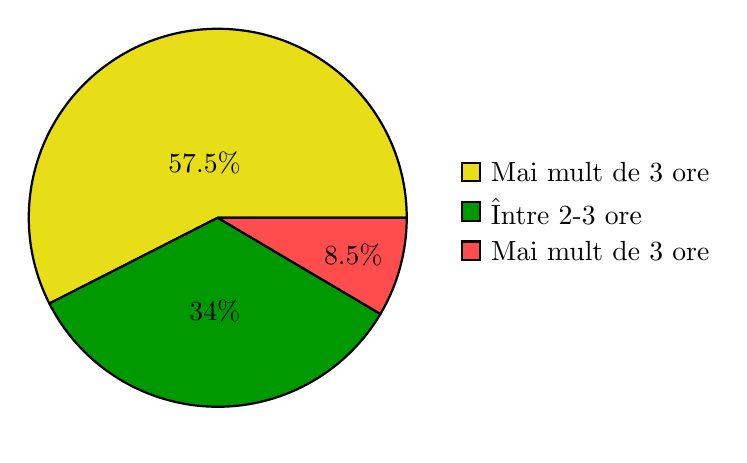
\begin{tikzpicture}[scale=0.8]
					% We will draw the pie chart here
					
					\pie[
					,
					color = {
						yellow!90!black, 
						green!60!black, 
						red!70},
					text = legend
					]
					{57.5/Mai mult de 3 ore,
						34/Între 2-3 ore,
						8.5/Mai mult de 3 ore}
						  
				\end{tikzpicture}
				\caption{Repartiția respondenților după numărul mediu de ore petrecut online } 
			\end{figure}
		\item  Referitor la nivelul de studii absolvit al respondenților (vezi figura 3.2), eșantionul nostru este format  preponderent de absolvenți de studii superioare (mai exact 61,3\%), restul fiind în prezent studenți. Mai mult, din tot eșantionul 22,6\% au studii post-universitare.
		\begin{figure}[!htb]
			\centering
			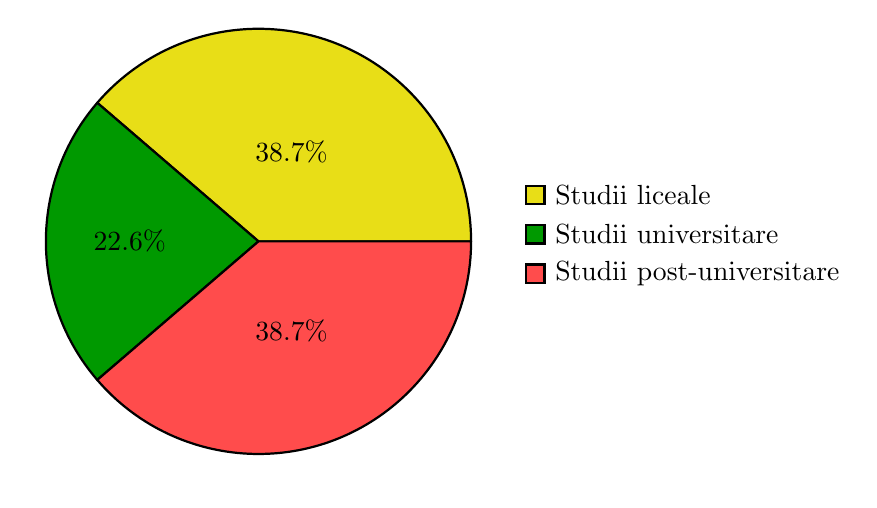
\begin{tikzpicture}[scale=0.9]
				% We will draw the pie chart here
				
				\pie[
				color = {
					yellow!90!black, 
					green!60!black, 
					red!70},
				text = legend
				]
				{38.7/Studii liceale,
					22.6/Studii universitare,
					38.7/Studii post-universitare}
				
			\end{tikzpicture}
			\caption{Repartiția respondenților după nivelul de studii absolvit} 
		\end{figure}
		\item Din perspectiva genului, marea majoritate a respondenților sunt de gen feminin, cu un procent de 90,6\% care indică faptul că femeile sunt mai empatice pentru a răspunde la chestionare online deoarece studiile analizate anterior nu au indicat nicio diferența atât de mare între cele două sexe, formându-se un echilibru între cele două genuri. Astfel, acest lucru nu înseamnă că bărbații achiziționează mai puțîn in mediul online, deoarece numărul scăzut de respondenți de gen masculin reflectă doar o limita a cercetării noastre și nu o realitate.
		\end{itemize}
	\qquad Pentru următoarea parte a lucrării, vom analiză principalele constatări ale
	eșantionarii populației, luând în considerare cele trei obiective definite anterior.
	\begin{enumerate}[(A)]
		\item\textbf {Primul obiectiv al studiului nostru}: să identificăm ce determina consumatorii online, tineri și educați din România să achiziționeze din mediul online și cum se informează.
		
		\qquad Pentru a identifica motivele pentru care cumpărătorii preferă să achiziționeze din mediul online și care este atitudinea lor față de beneficiile achizițiilor online, am adăugat o întrebare cu 5 itemi de răspuns (Posibilitatea de a realiza comparații, Accesibilitatea 24/24, Oportunitatea de a plăti un preț mai mic, Acces la gama mai largă de produse, Abilitatea de a împărtăși experiențe pe rețelele de socializare), unde respondenții trebuiau să măsoare pe o scară de la 1 la 5 gradul de acord al fiecărui item în parte(vezi întrebarea 4 - Anexă 1). Răspunsurile primite sunt reprezentate mai jos(vezi tabelul 3.1).
		\newcolumntype{M}[1]{>{\centering\arraybackslash}m{#1}}
	\bigskip
	\bigskip
					
			\begin{tabular}{ | M{12em} | M{1.2cm}| M{1.0cm} | M{1.2cm}| M{1.2cm} | M{2.2cm} | } 
				\hline
		& \multicolumn{5}{c|}{\textbf{Gradul de acord cu afirmația }} \\
				\hline
				\centering
				 
				& 1 Deloc & 2      Mic & 3 Mediu & 4 Mare & 5 \qquad Foarte mare \\ 
				\hline
				Posibilitatea de a realiza comparații & 2,8\% & 10,4\%  & 28,3\% & 22,7\% &35,8\%   \\ 
				\hline
				Accesibilitatea 
				24/24  & 2,8\%  & 0,9\%  & 19,8\% &19,8\%  & 55,7\% \\ 
				\hline
				Oportunitatea de a plăti un preț mai mic & 0,9\% & 6,5\%  &20,8\%  &20,8\% & 51\%  \\ 
				\hline
				Acces la o gamă mai largă de produse &0\%  &4,7\%  & 16\%  & 23,6\% & 55,7\% \\ 
				\hline
				Abilitatea de a împărtăși experiența online &33\%  & 13,2\%  &22,7\%  &16\% &14,1\% \\
				\hline		
			\end{tabular}
	\captionof{table}{Repartiția respondenților după răspunsurile la întrebarea "In ce masura conteaza pentru tine beneficiile achizitiilor online, mentionate mai jos?" } \label{tab:title} 
	\bigskip	

	\qquad Așadar, prin răspunsurile obtinuțe la această intrebare( vezi Tabelul 3.1.) putem deduce urmatoarele:
	\begin{itemize}
		\item \textit{accesibilitatea 24/24} și \textit{accesul la o gama mai largă de produse}  (ambele deținând un procent de 55,70\%) sunt principalele beneficii pentru care consumatorii online din România obișnuiesc să achiziționeze din mediul online , avantaje ce deosebesc magazinele virtuale de cele tradiționale.
		\item Următorul beneficiu care a fost ales de către 51\% dintre respondenți, se referă la \textit{oportunitatea de a plăti un preț mai mic} deoarece magazinele online nu au anumite costuri precum chiria spațiului și a utilităților, fapt ce reprezintă un mare plus pentru cumpărători.
		\item  Pe de altă parte, cel mai puțin important beneficiu al comerțului electronic ales de respondenți a fost \textit{abilitatea de a împărtăși experiență online}, ceea ce indică faptul că împărtășirea experienței personale nu reprezintă un avantaj al magazinelor virtuale, deoarece consumatorii tineri și educați din România își comunica experiențele prin alte metode.
	\end{itemize}
	
	\qquad Pentru a identifica sursele de informare pe care se bazează consumatorii online în momentul în care vor să realizeze achiziții online, am introdus 4 itemi ( Experiență personală, Review-urile de pe site, Opiniile celor apropiați, Informația oferită de motoarele de căutare), prin care respondenții au putut acordă o notă de la 1 la 5 (în ordine crescatoarea a acordului pe care o simte fiecare subiect asupra itemului respectiv)(vezi Întrebarea 5 Anexă 1). Răspunsurile sunt prezentate mai jos(Vezi tabelul 3.2).	
\bigskip
	\newcolumntype{M}[1]{>{\centering\arraybackslash}m{#1}}
	\begin{center}
		
		\begin{tabular}{ | M{13em} | M{1.1cm}| M{1.0cm} | M{1.1cm}| M{1.1cm} | M{2.2cm} |} 
			\hline
			&  \multicolumn{5}{c|}{\textbf{Gradul de acord cu afirmația} } \\
			
			\hline
			&  1 Deloc & 2 Mic & 3 Mediu & 4  Mare & 5 \qquad Foarte mare\\ 
			\hline
			Experiența personală  & 2,8\% & 1,9\% &10,4\%  & 28,3\% & 56,6\% \\ 
			\hline
			Review-urile de pe site  &0,9\%  &5,7\%   &27,4\%  &39,6\%  &26,4\%\\ 
			\hline
			Opiniile celor apropiați & 3,7\% & 3,7\%  & 29,2\%  & 35,8\% & 26,4\% \\ 
			\hline
			Informația oferită de motoarele de cautare & 9,4\% &10,4\%  &34,9\%  &34,9\% & 10,4\% \\ 
			\hline
		\end{tabular}
	\captionof{table}{Repartiția respondenților după răspunsurile la întrebarea "În ce masură ești influențat de factorii de mai jos atunci când realizezi achiziții online? "} \label{tab:title} 
	\bigskip
		
	\end{center}
	\qquad Conform datelor culese, (vezi Tabelul 3.2), în momentul achiziției unui produs online, consumatorii se bazează cel mai mult pe\textit{ experiență personală} din trecut, dețînând cel mai mare procent (84,9\%),urmând apoi cu un procent de 66\% \textit{review-urile de pe site}. Acest fapt denotă un aspect neașteptat și anume o încredere mai mare asupra review-urilor online decât in opiniile celor apropiați, ce poate fi explicat prin obiectivatea de care vor să dea dovadă tinerii cumpărători. Cel mai mic procent (45,3\%) l-a obținut informația oferită de motoarele de căutare,acest lucru putând fi datorat fie volumului mare de date disponibile online, fie gradului scăzut de acuratețe a informației prezente pe internet.
	
	\qquad Pentru a identifica elementele care contează cel mai mult pentru consumator atunci când ia decizia de a alege un magazin online în detrimentul altuia, am introdus o întrebare cu 5 itemi(Brand-ul produsului, Ușurință utilizării site-ului, Politică de Return, Diversitatea gamei de produse, Posibilitatea de a urmări comandă realizată), prin care respondenții au putut acordă o notă de la 1-5 în ordinea crescătoare a acordului pe care o simte fiecare subiect asupra item-ului respectiv(vezi întrebarea 6 Anexă 1). Răspunsurile sunt prezentate mai jos.(vezi tabelul 3.3)
\bigskip
	\newcolumntype{M}[1]{>{\centering\arraybackslash}m{#1}}
		\begin{center}
		\begin{tabular}{ | M{12em} | M{1.1cm}| M{1.0cm} | M{1.1cm}| M{1.1cm} | M{2.2cm} |} 
			\hline
			& \multicolumn{5}{c|}{\textbf{Gradul de acord cu afirmația} } \\
			\hline
			& 1 Deloc & 2 Mic & 3 Mediu & 4  Mare & 5 \qquad Foarte mare\\ 
			\hline
			 Brand-ul produsului &1,9\%  &10,4\%  & 41,5\%  &21,7\% &24,5\% \\ 
			\hline
		     Usurința utilizării site-ului& 3,8\% & 3,8\%   &17\%  &37,7\%  &37,7\% \\ 
			\hline
			Politica de Return & 5,7\%  &9,4\%  &18,9\%  &33\% &33\% \\ 
			\hline
			Diversitatea gamei de produse & 0,9\%  &2,8\%  &13,2\%  &33\% &50\% \\ 
			\hline
			Posibilitatea de a urmări comanda realizată & 2,8\%  & 6,6\%  &18,9\%  &32,0\% &39,6\% \\
			\hline
		\end{tabular}
	\captionof{table}{Repartiția respondenților după răspunsurile la întrebarea "In ce masura conteaza elementele enumarate mai jos atunci cand alegi un magazin online?" } \label{tab:title} 
	\bigskip
		
		\end{center}
		\qquad Potrivit raspunsurilor primite, am obținut următoarele rezultate:
		\begin{itemize}
			\item Jumătate din totalul de respondenți au oferit grad maxim item-ului privind \textit{diversitatea gamei de produse}, acesta având și cel mai mare procent (83\%), rezultat ce denotă atracția cumpărătorului online tânăr și educat față de un magazin mixt  în locul unuia specializat pe o singură gama de produse. Acest lucru se datorează faptului că procesul de achiziție a consumatorului se simplifică, acesta având posibilitatea de a cumpără mai multe produse dintr-un singur loc și dovedind abilități de organizare și eficientizare a achizițiilor.
			\item Pe următorul loc, cu procentul de 75,4\%, este \textit{ușurință utilizării site-ului} element ce determina importantă nivelului de accesibilitate al paginii web pentru consumatorii tineri și educați care obișnuiesc să achiziționeze online cele mai bune oferte găsite.
			\item Un alt aspect interesant este faptul că \textit{Politică de return }are un scor mediu (66\%), fapt ce pune la îndoială informațiile pe care le au consumatorii tineri și educați cu privire la drepturile lor privind returnarea bunurilor achiziționate. 
			\item De asemenea, contrar așteptărilor, elementul cu cele mai puține voturi îl reprezintă \textit{brand-ul produsului} având un procent de doar 46,2\%, care indică faptul că, în prezent, consumatorii online nu mai pun cel mai mare accent pe notorietatea  magazinului de la care cumpără, ci se focusează pe alte elemente în procesul decizional, precum cele amintite anterior.
		\end{itemize}
		
		\quad  Referitor la nivelul de documentare a consumatorilor înaintea plasării unei comenzi online, am introdus o întrebare cu un singur item prin care respondenții au putut acordă o notă de la 1 la 5 în ordinea crescătoare a acordului cu care se informează.
		
		\begin{figure}[!htb]
			\centering
			\includegraphics[width=14cm, height=5cm]{"figures/trei.png"}
			\caption{ Repartizarea respondenților după nivelul de documentare a respondenților înainte de a comanda online}\label{fig:unuspre}
		\end{figure}
	
	 	\qquad Așadar, prin răspunsurile oferite se observă că respondenții  au un nivel crescut de maturitate, alegând să se informeze riguros înainte de a alege să cumpere un produs, deoarece  35,8\% au ales că se informează mult, iar 43,4\%, aproape jumătate, au ales chiar grad maxim de informare. Acest lucru este subliniat și de faptul că doar 2,8\% din respondenți au ales cea mai mică notă (1) care înseamnă informare deloc. Astfel, se observă o creștere a nivelului de educație al consumatorilor tineri și educați din România prin atenția pe care o oferă cumpărăturilor în mediul online.

	 	
		\item \textbf{Al doilea obiectiv al studiului nostru }: să identificăm categoriile de produse și frecvența achizițiilor online.
		
		\qquad Pentru a identifica categoriile de produse cele mai achiziționate în mediul online, am propus acestora să răspundă care e categoria de produse pe care o cumpără cel mai des online.(vezi întrebarea 7 Anexă 1).
		\begin{figure}[!htb]
			\centering
			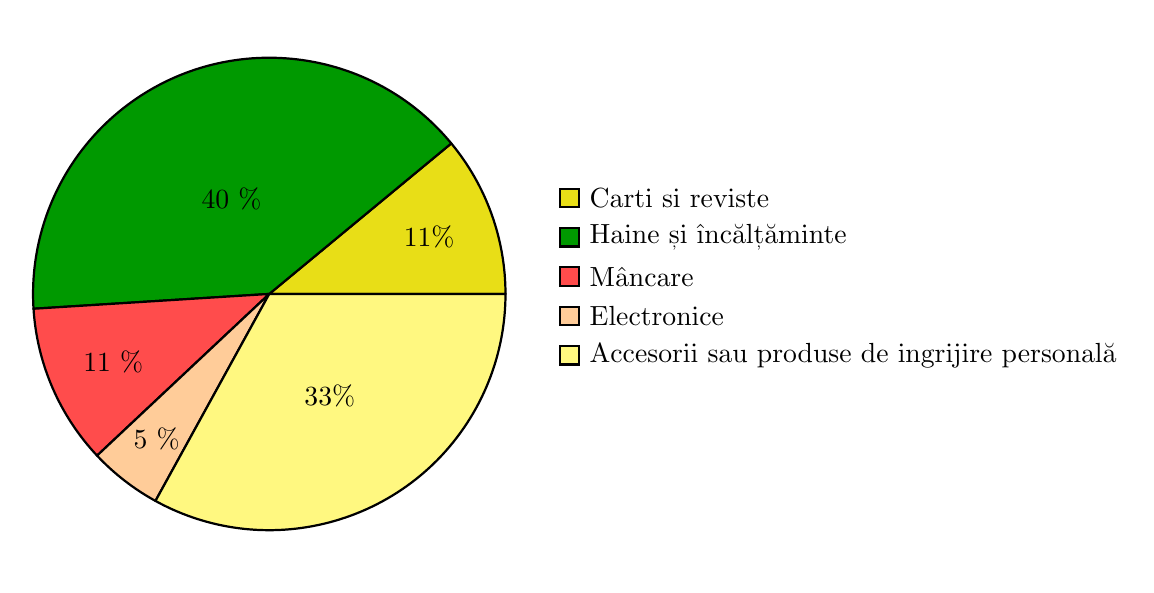
\begin{tikzpicture}
				% We will draw the pie chart here
				
				\pie[
				color = {
					yellow!90!black, 
					green!60!black, 
					red!70,
					orange!40,
					yellow!50 },
				text = legend
				]
				{11/Carti si reviste,
					40 /Haine și încălțăminte,
					11 /Mâncare,
					5 /Electronice,
					33/ Accesorii sau produse de ingrijire personală}
				
			\end{tikzpicture}
			\caption{Repartiția respondenților după categoria cea mai achiziționată în perioada februarie -aprilie 2021} 
		\end{figure}
	
		\qquad Cei mai mulți dintre respondenți ( vezi figura 3.4) au răspuns că\textit{ hainele și încălțămintea} reprezintă cea mai frecvența categorie de produse achiziționată. Pe locul doi se află \textit{accesoriile/ produsele de îngrijire personală}, iar pe trei,\textit{ cărțile și revistele} aflându-se la egalitate cu \textit{mâncarea}. Aceste categorii de produse au fost bunurile cel mai frecvent achiziționate online de către  consumatorii online, tineri și educați din România în perioada februarie-aprilie 2021.
	
		\qquad Pentru a cunoaște frecvența  cu care consumatorii achiziționează, în mediul  online, am propus acestora să răspundă cât de frecvent obișnuiesc ei să achiziționeze produse sau servicii cu ajutorul internetului fie de pe laptop/telefon sau tabletă(vezi întrebarea 8, Anexă 1)
		\begin{figure}[!htb]
			\centering
			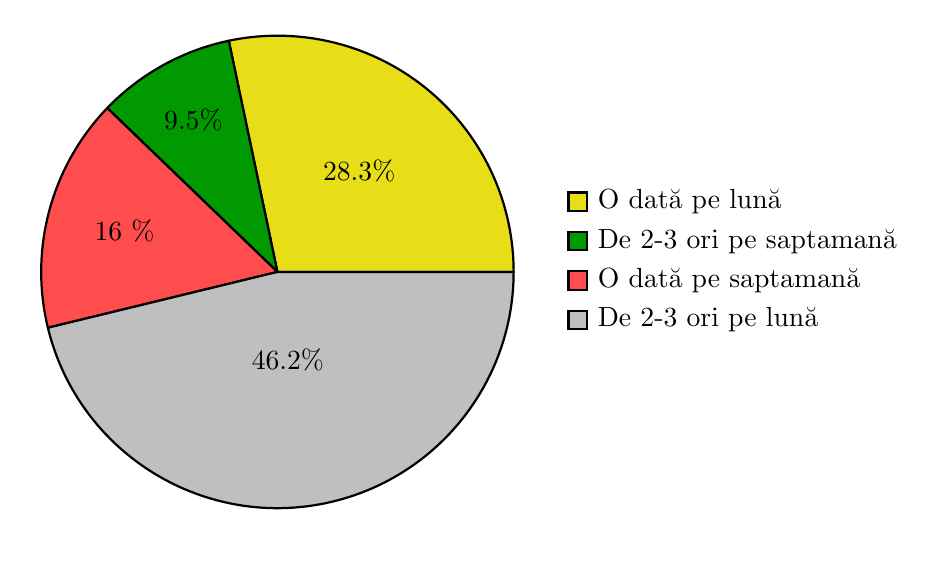
\begin{tikzpicture}
				% We will draw the pie chart here
				
				\pie[
				color = {
					yellow!90!black, 
					green!60!black, 
					red!70,
					gray!50},
				text = legend
				]
				{28.3/O dată pe lună,
					9.5/De 2-3 ori pe saptamană,
					16 /O dată pe saptamană,
					46.2/De 2-3 ori pe lună}
				
			\end{tikzpicture}
			\caption{Repartiția respondenților după categoria cea mai achiziționată în perioada februarie-aprilie 2021} 
		\end{figure}
	
\newpage
		\qquad Conform răspunsurilor culese,(vezi Figura 3.5) cei mai mulți respondenți (46,2\%) au spus că achiziționează de \textit{2-3 ori pe luna}, fapt ce se încadrează că o medie între des și rar, iar cei mai puțini respondenți (9,4\%) au spus că achiziționează de \textit{2-3 ori pe săptămână}. Acest fapt ne poate induce ideea că consumatorii online, tineri și educați din România nu au integrat achizițiile online în cumpărăturilor lor de zi cu zi. Astfel, putem înțelege că ei obișnuiesc să achiziționeze în mediul digital doar anumite produse sau servicii care nu se regăsesc în magazinele fizice.
\bigskip	
		\item \textbf{Al treilea obiectiv al studiului nostru}: Să identificăm problemele apărute și comportamentul post-achiziție al consumatorilor online tineri și educați din România.
	\end{enumerate}		
	\quad Pentru a află ce tip de probleme au întâmpinat atunci când au achiziționat un produs online, am adăugat o întrebare cu 5 itemi (Timpul de livrare nu a fost respectat, Produsul a ajuns cu defecte, Au fost costuri mari cu livrarea, Calitate inferioară, Returnarea produsului a fost dificilă) prin care respondenții au putut acordă o notă de la 1-5 în ordinea crescătoare a acordului pe care o simte fiecare subiect asupra item-ului respectiv(vezi întrebarea 10, Anexă 1). Răspunsurile sunt prezentate mai jos(vezi tabelul 3.4).
	\newline
	
\bigskip		
		\newcolumntype{M}[1]{>{\centering\arraybackslash}m{#1}}
		\begin{center}
			\begin{tabular}{ | M{14em} | M{1.1cm}| M{1.0cm} | M{1.1cm}| M{1.1cm} | M{2.2cm} |} 
				\hline
				& \multicolumn{5}{c|}{\textbf{Gradul de acord cu afirmația} } \\
				\hline
				& 1 Deloc & 2 Mic & 3 Mediu & 4  Mare & 5 \qquad Foarte mare\\ 
				\hline
				Timpul de livrare nu a fost respectat  &8,5\%  &37,7\%  &27,4\%  &18,9\% &7,5\% \\ 
				\hline
				Produsul a ajuns cu defecte &34\%  &44,3\%   &17\%  &4,7\%  &0\%\\ 
				\hline
				Au fost costuri mari cu livrarea &13,2\%  & 26,4\%  &29,2\%  &18,9\% &12,3\% \\ 
				\hline
				Calitate inferioară &18,9\%  &41,5\%  & 24,5\%  &12,3\%  &2,8\% \\ 
				\hline
				Returnarea produsului a fost dificilă & 32,6\%  & 27,4\%  & 18\% & 9,4\% &5,7\% \\
				\hline
			\end{tabular}
		\captionof{table}{Repartiția respondenților după răspunsurile la întrebarea "în ce masură ați întâmpinat problemele de mai jos atunci când ați comandat un produs de pe internet?" } \label{tab:title} 
		
		\end{center}
	\qquad\space\space Potrivit datelor culese(vezi tabel 3.4), consumatorii online tineri și educați nu au prea întâlnit acest tip de probleme atunci când au plasat o comandă online, fapt dovedit de notele mici acordate problemelor din figura de mai sus. Cea mai întâlnită, dar care tot deține un scor nu foarte mare (31,2\%) este \textit{costuri mari cu livrarea}, urmând pe locul doi, cu un procent de 26,4\%, \textit{timpul de livrare care nu a fost respectat} fapt ce subliniază importantă calității livrării bunurilor în procesul de achiziție online. Problema întâlnită cel mai puțin a fost \textit{Produsul a ajuns cu defecte} având un procent de aproape 5\%.
	
	\quad Pentru a identifica cum reactioneaza consumatorii  online atunci cand intalnesc o problema cu produsul livrat de la un magazin online, am intrebat cum au actionat ei dupa ce au constat ca bunul primit in urma comenzii, nu este conform cerintelor lor. Raspunsurile sunt prezentate mai jos(vezi figura 3.6).
	\begin{figure}[!htb]
		\centering
		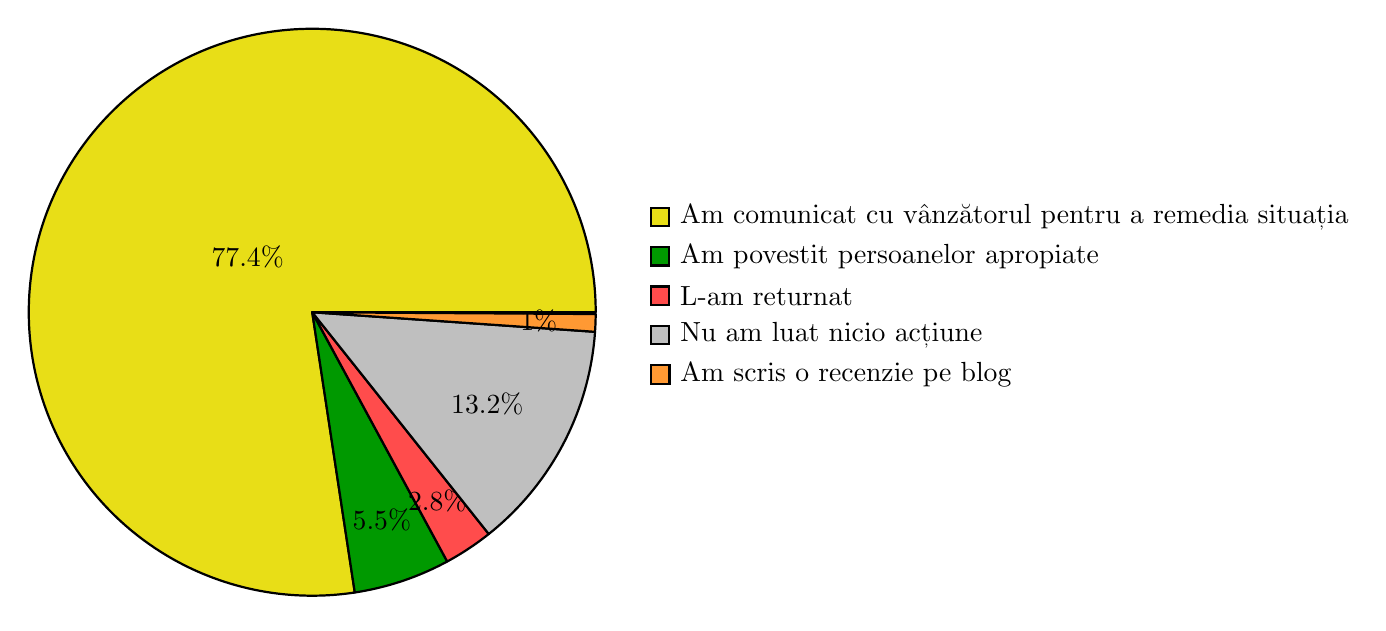
\begin{tikzpicture}[scale=1.2]
			% We will draw the pie chart here
			
			\pie[
			color = {
				yellow!90!black, 
				green!60!black, 
				red!70,
				gray!50,
				orange!80},
			text = legend
			]
			{77.4/Am comunicat cu vânzătorul pentru a remedia situația,
				5.5/Am povestit persoanelor apropiate,
				2.8/L-am returnat,
				13.2/Nu am luat nicio acțiune,
				1/Am scris o recenzie pe blog}
			
		\end{tikzpicture}
		\caption{Repartiția respondenților dupa problemele pe care le-au intalnit în achiziția unor produse online} 
	\end{figure}

	\quad Conform răspunsurilor obținute, am constat că cei mai mulți respondenți, anume un procent de 77,4\% din total au răspuns că ei comunica problema întâlnită vânzătorului/ magazinului de la care a achiziționat bunul pentru a putea remedia și rezolva situația creată, fapt ce subliniază încă o dată seriozitatea și încrederea de care da dovadă consumatorul online și tânăr față de achizițiile din mediul online. Acest lucru evidențiază profilul stabilit al participanților, la acest studiu, încă de la începutul cercetării. Din păcate, au existat și persoane (13,20\%) care au ales să nu ia nicio acțiune cu privire la bunul achiziționat și neconform cerințelor și asteparilor lor. Au existat și câteva păreri, în minoritate, care au ales să acționeze diferit și unic precum: împărtășirea experienței celor apropiați(5,5\%), returnarea produsului (2,8\%) și scrierea experienței pe un blog (0,9\%).
	
	\quad  În ultima parte a analizei datelor culese doresc să integrez întrebările deschise de la finalul chestionarului (vezi întrebarea 12 și 13, Anexă 1) alături de celelalte întrebări pentru a crea un profil al respondenților bazat pe cele 3 categorii de vârstă (18-21, 22-24, 25-30) și pentru a putea identifica diferențele ce pot apărea între segmentele de clienți, în funcție de categoria de vârstă.
	
	\quad În cadrul întrebările deschise, privind experiențele consumatorilor, am dorit să vedem ce consideră  el că fiind cea mai bună experiență în mediul online și problemele care l-au determinat să vadă o altă experiență, drept cea mai puțin bună.
	
	\quad Faptul că procentul răspunsurilor feminine excede procentul răspunsurilor masculine poate indica faptul că femeile sunt mai deschise la răspunderea de chestionare online decât bărbații, acest lucru reprezentând doar o limită al cercetării noastre.

	\quad Din procentul de 90,6\% din totalul persoanelor de gen feminin care au răspuns la chestionar, 33\% dintre respondenții au vârsta cuprinsă între 18-21 de ani( abia au terminat studiile liceale sau sunt studente la o facultate), 29\% au vârstă cuprinsă între 22-24 ( sunt absolvente de licență sau studente la master), 38\% au vârstă cuprinsă între 25-30 de ani (fie sunt absolvente de studii superioare sau studente la doctorat)(vezi figura 3.7).
	\begin{figure}[!htb]
		\centering
		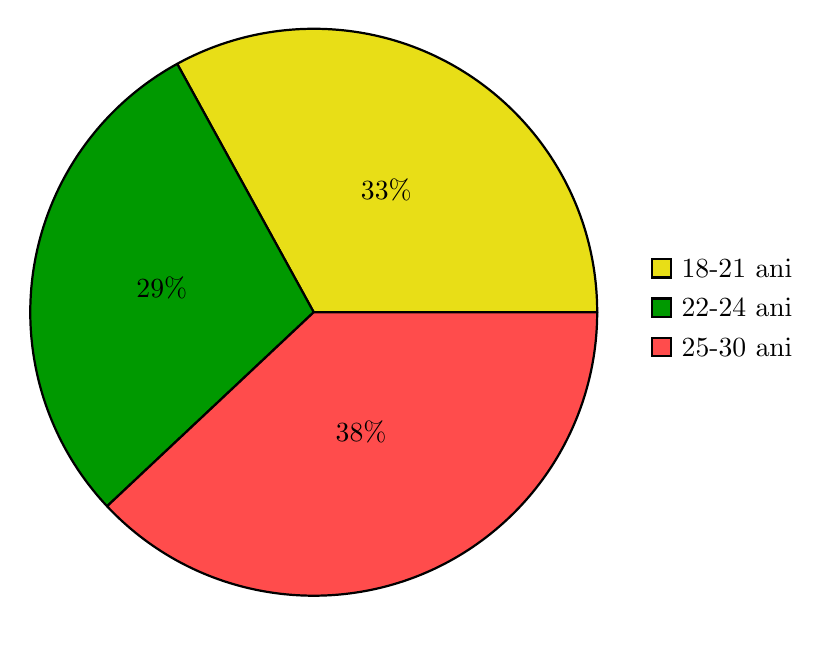
\begin{tikzpicture}[scale=1.2]
			% We will draw the pie chart here
			
			\pie[
			color = {
				yellow!90!black, 
				green!60!black, 
				red!70},
			text = legend
			]
			{33/18-21 ani ,
				29/22-24 ani,
				38/25-30 ani}
			
		\end{tikzpicture}
		\caption{Repartiția respondenților după problemele pe care le-au întâlnit în achiziția unor produse online} 
	\end{figure}
\newpage		
	\begin{itemize}
		\item \textbf{Respondenții de gen feminin cu vârsta cuprinsă în intervalul 17–21 ani} reprezintă 33\% din totalul de respondenți de gen feminin. În  urmă analizei asupra datelor oferite, am extras informațiile relevante pentru a putea sublinia caracteristicile acestei categorii. 
		
		\quad Primul lucru pe care l-am sesizat a fost faptul că 57\% dintre respondenții acestei categorii petrec mai mult de 3 ore online, înafara cursurilor de la facultate, însă frecvența cu care comandă online este redusă, procentul de  37\% spunând că plasează comenzi o dată pe luna . Acest lucru relevă un paradox și anume, dacă o persoană petrece mult timp în mediul online nu înseamnă că își face cumpărăturile tot în acest mediu.
		
		\quad Următorul lucru pe care l-am identificat a fost faptul că\textit{ hainele și încălțămintea} reprezintă cea mai frecvența categorie de produse achiziționată online (50\% au ales această categorie),  fapt ce relevă încrederea pe care o au acești consumatori tineri în aceste magazine. Acest lucru este subliniat și de procentul ridicat de 68,8\% în care aceștia au răspuns că atunci când apar eventuale erori cu comandă sau produsul achiziționat au siguranță că pot comunica cu producătorul pentru a remedia situația ulterior. 
		
		\quad Pentru a analiza răspunsurile oferite de respondenți la întrebările deschise am decis să grupăm experiențele împărtășite pentru a le evidenția pe cele care s-au afirmat cel mai mult:
		\begin{itemize}
			\item În cazul întrebării deschise referitoare la cea mai bună experiență pe care au avut-o până acum, consumatorii au subliniat în mare parte avantajele pe care magazinele online le oferă cumpărătorilor și care contează cel mai mult pentru ei. Dintre acestea enumerăm: rapiditatea livrării produsului într-un timp cât mai scurt, fiind cel mai des menționat element, urmând apoi disponibilitatea producătorului de a răspunde și remedia eventuale erori și apoi posibilitatea de a urmări produsul achiziționat în timp real.
			\item 	În cadrul întrebării referitoare la experiență mai puțîn bună s-au accentuat problemele pe care consumatorii le-au întâlnit. Dintre acestea, cel mai mult s-au menționat timpul de livrare care nu a fost respectat și neconcordanță dintre calitățile promise în mediul online față de cele primite la momentul livarii produsului. 
		\end{itemize}
	
		\item \textbf{Respondenții de gen feminin cu vârsta cuprinsă în intervalul 22-24 ani} este reprezentată de 29\% din totalul de respondenți de gen feminin. În această categorie s-au sesizat mici diferențe, față de cea analizată anterior pe care le voi prezența în rândurile următoare.
		
		\quad Prima diferența pe care am sesizat-o la femeile e-consumator, cu vârstă cuprinsă între 22-24, este ideea că în ciuda faptului că petrec tot la fel de mult timp online că și generația anterioară, procentul de achiziții online cel mai mare (60\%) este la varianta cu 2-3 achiziții pe luna. Acest fapt ne indică că femeile sunt mult mai atente cu programul lor și că încearcă să-și organizeze cât mai eficient activitățile ce necesitau ore înainte în magazinele fizice, dar posibile doar cu un click în mediul online.
		
		\quad Următoarea diferența pe care am observat-o a fost la categoriile de produse achiziționate cel mai des online. Față de generația anterioară, respondenții de gen feminin din această categorie au un procent mai scăzut (42,9\%) la categoria de \textit{haine și încălțăminte}, urmat de \textit{accesorii și produse de îngrijire} cu un procent de 35,8\%. Acest lucru dezvăluie tendința fetelor de a pune mult mai mare accent pe îngrijirea personală cu înaintarea în vârstă. 
		
		\quad La întrebările deschise aflate la finalul chestionarului, fetele au menționat aproximativ aceleași elemente care s-au amintit, referitoare la experiențele pozitive și negative pe care le-au avut, în schimb, s-au sesizat câteva elemente de noutate precum:
		\begin{itemize}
			\item În cadrul celei mai bune experiențe s-a adăugat cererea de feedback din partea producătorului, existența unor costuri mai mici online și utilizarea site-urilor pentru comparații între produsele dorite drept elemente care ajută la încheierea cu succes a unui proces de achiziționare în mediul electronic.
			\item În cazul experienței mai negative s-a adăugat lipsa returnării sumei oferite pe achiziționarea produsului în urmă returnării acestuia, fapt ce constituie o mare problema în rândul consumatorilor de orice gen.
		\end{itemize}
	
		\item \textbf{Respondenții de gen feminin cu vârsta cuprinsă în intervalul 25-30 ani} reprezintă cel mai mult din totalul de respondenți de gen feminin și anume 38\%. În cadrul acestei analize am făcut o comparație între cele două generații prezentate anterior și generația care a devenit matură și trebuie să ofere mai multe atenție costurilor pe care le are.
		
		\quad În primul rând, persoanele de gen feminin cu vârstă între 25 și 30 de ani petrec la fel de mult timp online, acest lucru putând fi datorat job-ului care s-a transformat remote în contextul pandemiei Covid19, însă achiziționează mai mult decât prima categorie de vârstă, ceea ce relevă o stabilitate materială dar mai puțîn decât a două, fiind mult mai atente pe ce cheltuiesc banii câștigați din venituri proprii.
		
		\quad În al doilea rând, fetele/femeile din acest grup subliniază tendința pe care am observat-o și la generația anterioară privind accentul pe \textit{produsele de îngrijire personală} cu un procent de 43,5\%, iar locul 2 fiind ocupat, în acest caz, de categoria de \textit{haine și încălțăminte}. De asemenea, nouă categorie de produse (electrocasnicele)  introdusă de aceștia și procentul mare (69,5\%) obținut în vederea comunicării cu producătorul indiferent de problemele întâlnite, relevă o notă de maturitate venită odată cu creșterea în vârstă.
		
		\quad În ultimul rând, experiențele dezvăluite la întrebările deschise au expus noi caracteristici/elemente pe care consumatorii le doresc să le întâlnească sau nu precum:
		\begin{itemize}
			\item Elementele dorite și care vin în completarea celorlalte experiențe pozitive, amintite anterior, sunt suprizele sau produsele extra pe care unii producători le folosesc pentru a-și loializa clienții și  calitatea ridicată unor produse importante și vitale precum o piesă auto ce după spusele unei respondente a rezistat conform trăsăturilor menționate.
			\item Elementele care se doresc a fi evitate sunt reprezentate costurile mari cu transportul și nerespectarea timpului de livrare, însă în cazul acestui interval de vârstă, aceste achiziții au fost efectuate înafara țării, fapt ce îngreunează procesul de achiziție și livrare datorită taxelor vamale și distanței foarte mari dintre producător și destinatar.
		\end{itemize}
	\end{itemize}
\newpage	
	\subsection{Concluzii - studiu de caz}
	\qquad În urma cercetării realizate, avem un profil al comportamentului consumatorului online, tânăr și educat din România având în vedere elementele de care are nevoie pentru a achiziționa mai mult în mediul online dar și trăsături negative care încă nu-i oferă siguranța de a utiliza comerțul electronic. Astfel, concluzionam următoarele: \begin{enumerate}[1.] 
	\item Cele mai importante beneficii ale comerțului electronic evidențiate de respondenți sunt accesibilitatea 24/24 și livrarea rapidă a produselor alături de accesul la o gama mai largă de produse la prețuri mai avantajoase decât în magazinele fizice. 
	\item Experiența personală reprezintă sursa de baza în momentul în care un consumator tânăr și educat decide să-și achiziționeze un produs din mediul online, fapt ce suprinde datorită existenței unui volumul mare de informații disponibil pe motoarele de căutare, dar care, din păcate, reprezintă ultima să sursă de informare din diverse motive precum autenticitatea informațiilor disponibile, sursele de informare nu sunt adesea actualizate prezentului iar detaliile de pe site nu pot fi întotdeauna verificate. 
	\item Motivul pentru care unii consumatori, tineri și educați din România aleg un magazin electronic în detrimentul altuia este diversitatea gamei de produse, care ajută consumatorii online, români să-și eficientizeze productivitatea folosind un clik de pe un singur site.
	 \item Legat de măsura în care se documentează consumatorii online, tineri și educați înainte de a plasa o comandă, respondenții au evidențiat nivelul de educație crescut prin acordarea notei maxime, care înseamnă că sunt mult mai atenți cu produsele pe care le achiziționează și de unde le cumpără înainte de a plăti.
	\item În ciuda faptului că pandemia covid19 a restricționat accesul persoanelor în magazine și supermarket-uri, categoria de produse cea mai achiziționată online nu este mâncarea, ci hainele și încălțămintea, iar acest fapt se datorează gamei largi de produse de îmbrăcăminte ce poate fi găsită în magazinele virtuale și codurilor de reducere care se pot utiliza exclusiv online. 
	\item Analizând raportul dintre timpul petrecut online și frecvența achizițiilor online am constatat că nu există o regulă stabilită care să funcționeze deoarece am întâlnit în cadrul rezultatelor, persoane care petreceau mult timp online, însă numărul de achiziții depindea de categoria de vârstă în care se încadra respondentul. 
	\item S-a evidențiat drept cea mai importantă problema, costurile și timpul livrării produsului care nu îngreunează satisfacerea nevoilor cumpărătorilor. De asemenea, respondenții au afirmat că atunci când întâmpina probleme cu produsul achiziționat și livrat acasă, ei decid să comunice cu producătorul pentru a putea remedia situația în cel mai scurt timp posibil. 
	\end{enumerate} 

	\quad Profilul socio-demografic al consumatorilor online, tineri și educați din România participanți la sondajul de opinie realizat (eșantionul fiind de 106 persoane) este: majoritatea sunt persoane de gen feminin (90,6\%), de gen masculin fiind doar un procent de 9,4\%.  În rândul respondenților, 31,1\% au vârstă cuprinsă între 18-21 ani, 25,5\% au vârstă cuprinsă între 22-24 de ani, iar 26,4\% au vârste cuprinse între 25-30 de ani. Majoritatea respondenților chestionați sunt absolvenți de studii superioare de nivel licență sau masterat sau studenți ai acestor programe. 
	
	

	
	\newpage 
	\section*{Concluzii}
	\addcontentsline{toc}{section}{\textsc{Concluzii }}
	
	\qquad\qquad Tema acestei lucrări "Comportamentul consumatorului online tânăr și educat din România. Studiu de caz" este abordată pe parcursul a trei capitole care cuprind informații despre comportamentul unui consumator online, în general și în particular comportamentului consumatorului online tânăr și educat din România. De asemenea, este abordat specificul comerțului electronic, atât la nivel conceptual, cât și la nivel de Uniune Europeană dar și situația din România. La nivelul studiului de caz scopul urmărit a fost crearea unui profil al consumatorului online tânăr și educat din România pentru a ajuta firmele din comerțul electronic să înțeleagă mai bine comportamentul acestuia și să se plieze pe cerințele lui.
	
	\quad Potrivit datelor publicate de Parlamentul European de la Bruxelles,  comerțul electronic s-a dezvoltat din ce în ce mai mult în ultimii ani, iar acest lucru a fost evidențiat prin faptul că acesta devenit o componentă importantă a sistemului de afaceri. De asemenea, comerțul electronic cuprinde atât tranzacții cu bunuri tangibile, cât și tranzacții privind bunurile intangibile. Astfel, consumatorii online au oportunitatea de a alege dintr-o gama mai largă de opțiuni oferite de magazinele digitale, iar managerii au oportunitatea de a analiza informațiile oferite de consumator, transformând aceste date direct în strategii de marketing. 
	
	\quad Pentru a analiza comportamentul consumatorului online a fost necesar să înțelegem comportamentul consumatorului, în general, concluzionând că întotdeauna la baza oricărui tip de comportament al cumpărătorului există un individ sau un grup, conceptul de a satisface o nevoie și un proces care duce la o decizie. Am explicat atenția pe care întreprinderile trebuie să o oferă relației dintre consumator și producător prin cadrul unui sistem numit Managementul relațiilor cu clienții. Conform teoriei lui Koetler, am identificat tipurile de decizii pe care un consumator le poate lua, fie că au loc în mediul online sau în magazinele fizice, apoi am completat cu cele trei modele de marketing care fac legătură dintre utilizarea tehnologiei și comportamentul consumatorului pentru a înțelege evoluția comerțului electronic. De asemenea, am considerat relevant de adus în discuție și importanța generațiilor de consumatori, fapt ce ne-a ajutat să identificăm cum se raportează la  tehnologie, fiecare consumator, în funcție de generația din care face parte.
	 
	\quad În continuarea analizei teoretice asupra comportamentului consumatorului online am observat că datorită multitudinii de posibilități care i se oferă, în mediul virtual, acesta este nevoit să ia în considerare anumite elemente mai importante pentru achiziționarea unui produs în detrimentul altuia. Acești factori i-am putea împărți în două categorii: factori ce țin de persoană consumatorului precum constrângerile de timp, motivația cumpărării, nivelul de informare și factori ce țin de magazinul digital precum accesibilitatea site-ului, securitatea informațiilor, calitatea oferită de magazin și altele. Procesul de cumpărare al consumatorului online nu se diferențiază cu mult de cel al consumatorului fizic deoarece la baza există același etape, doar cu mențiunea că acestea au loc exclusiv online. Cumpărătorul acum va caută informația online cu ajutorul motoarelor de căutare și va apela mult mai ușor la review-uri. Va putea compara și analiza informația utilizând instrumente de sortare și filtrare a datelor, iar luarea deciziei va avea loc numai după ce consumatorul este conștient de riscurile posibile. În cazul mediului online, mecanismul de reclamații poate fi un proces mult mai greu, unii utilizatori alegând să nu mai remedieze situația cu producătorul. Interacțiunile post-vânzare sunt facilitate de mediul online, oferind posibilitatea de loializare a clienților prin email-uri de promovare. La fel că orice alt proces, achiziționarea de produse online are atât avantaje cât și dezavantaje. Avantajul cel mai important îl reprezintă accesul la o varietate mai largă de produse, iar cel mai mare dezavantaj este livrarea unui produs cu o calitate inferioară.
	
	\quad  Ca urmare a specificului comportamentului consumatorului online, există studii și cercetări deja publicate. În urma cercetării secundare, am analizat trei studii de caz  dintre care, două au fost realizate în 2013, iar unul în  2016 asupra situației din România privind achizițiile online și comportamentul consumatorului online tânăr și educat, iar astfel concluzionăn următoarele: Piață de comerț electronic din România este în strânsă legătură cu accesul la Internet, iar având în vedere că rata de penetrare pe Internet era scăzută față de media Uniunii Europene, mediul online este accesat doar de o parte din populație, fapt ce îngreunează dezvoltarea comerțului  în mediul digital. Datorită creșterii nivelului de educație, s-a dovedit că nouă generație de tineri este mult mai familiarizată cu tehnologia online și este mai dispusă să se confrunte cu riscurile percepute de mediul virtual. Cele mai achiziționate categorii de produse de românii care achiziționează online sunt electronicele, îmbrăcămintea și produsele de frumusețe și îngrijire personală. Un alt factor care a influențat dezvoltarea comerțului electronic în România este pandemia Covid19, care a dus la o creștere a cumpărăturilor online în rândul românilor. 
	
	\quad De asemenea, am realizat și o comparație între trei cercetări care au abordat tema comportamentului consumatorului online din România într-un mod unic. Dacă ar fi să comparăm rezultatele obținute în cadrul studiului de caz și rezultatele obținute în cercetările prezentate putem constata că: între prima cercetare și rezultatele noastre există un mic dezacord între factorii care determina cumpărătorii să achiziționeze online și anume în cercetarea din 2016, a lui Onete Bogdan,  a reieșit că românii pun mare accent pe brand-ul și imaginea unui brand pe când în răspunsurile oferite de respondenți s-a observat că acest element nu mai reprezintă o importanță așa mare, însă consumatorii români care au răspuns atunci și cei care au răspuns acum au evidențiat importanța prețului și a livrării drept factor care le influențează procesul decizional; O altă cercetare, care a subliniat elemente comune, a fost Cercetarea din 2013, a Claudiei Bobalca, care a scos în evidență avantajele și dezavantajele achizițiilor online. Putem spune, că în mare parte, beneficiile și problemele rezultate din întrebările deschise și închise ale chestionarului s-au regăsit și în cercetarea din 2013 realizată de Claudia Bobalca, că de exemplu avantaje precum comoditatea livrării sau accesibilitatea 24/24 pentru a cumpără un produs online și diversitatea gamei de produse în mediul digital, dar și dezavantaje privind timpul livrării produselor sau costurile prea mari cu transportul.
	
	\quad Studiul de caz al acestei lucrări se găsește în cadrul celui de-al treilea capitol, având la baza o cercetare primară, cantitativă ce relevă motivele pentru care cumpărătorii online, tineri și educați din România cumpără din mediul digital, ce categorii de produse achiziționează și cum reacționează la problemele apărute. Scopul acestui studiu de caz a fost realizarea profilului consumatorului online tânăr și educat din România pentru a oferi informații firmelor prezente în mediul online care țintesc acest tip de consumator în strategiile lor. Studiul de caz are la baza o cercetare primară cantitativă, metodă folosită fiind sondajul de opinie. Instrumentul folosit a fost chestionarul lansat online prin intermediul aplicației Google Forms, în perioada 27 aprilie- 4 mai 2021, având un număr de 106 răspunsuri valide.
	
	\quad  Noțiunile teoretice prezentate pe parcursul celor două capitole anterioare au reprezentat baza definirii scopului și obiectivelor studiului de caz și implicit în procesul de realizare a chestionarului cu ajutorul căruia au fost culese datele primare.
	
	\quad Concordanța dintre elementele care au rezultat din cercetarea secundară  pe parcursul capitolului 2 și datele obținute în urmă cercetării primare este vizibilă. Astfel, potrivit datelor culese în urmă chestionarului lansat concluzionam că anumite aspecte privind comportamentul consumatorului online tânăr și educat din România s-au păstrat de-a lungul dezvoltării comerțului electronic precum motivul pentru care aleg să achiziționeze și anume oportuntiatea unei game mai largi de produse, alegerea unui produs în urmă experienței personale și nu a opiniilor altor consumatori online, cea mai achiziționată categoria de produse online a rămas tot îmbrăcămintea și încălțămintea. De asenmenea, există și anumite aspecte care s-au schimbat și îmbunătățit precum creșterea nivelului de informare înainte de a cumpăra un produs online, fapt ce relevă statutul educațional ridicat, iar acest lucru este subliniat și de comportamentul responsabil al consumatorului online tânăr și educat care alege să discute cu comerciantul pentru a remedia problemele ce apar.
	
	\quad Concluzionând subiectul tratat, pe parcursul acestor pagini, îl putem descrie ca fiind o tema complexă și de actualitate și în același timp interesantă și inovatoare pentru domeniul marketing-ului online și marketing-ului în general. Urmărirea modului în care se dezvoltă comportamentul consumatorului online, tânăr și educat din România în concordanță cu dezvoltarea comerțului electronic rămâne un subiect instigator ce aduce în permanență noi oportunități de cercetare și asta deoarece companiile doresc identificarea și satisfacerea nevoilor consumatorilor online în așa fel încât aceștia să fie atrași cât mai mult în a cumpăra produsele acestora online.
	\newpage
	
	\section*{Referințe bibliografice}	
\addcontentsline{toc}{section}{\textsc{Referințe bibliografice}}
\space
\bigskip
\bigskip
	
	\textbf{Cărți în format electronic:}
	\begin{enumerate}[1.]
	\item Armstrong Gary, Adam Stewart, Denize Sara, Kotler Philip, 2012,\textit{Principles of martketing}, Pearson.
	\item Babin J. Barry, Harris G., 2017, \textit{CB Consumer Behaviour}, Nelson Education.
	\item Șandor Dan Sorin, 2013, Metode și Tehnici de Cercetare în Științele Sociale, Tritonic books.
	\end{enumerate}
	\textbf{Articole științifice în format electronic:}
	\begin{enumerate}[1.]
		\item Anastasiei Bogan, Dospinescu Nicoleta. 2019.\textit{Electronic Word-of-Mouth for Online Retailers:Predictors of Volume and Valence}
		\item Bighiu Georgiana, Adriana Manolică, Roman Teodora Cristina. 2015.\textit{Compulsive buying behavior on the internet}
		\item Bobalca Claudia. 2015. \textit{The Loyal Customers’ Perception Regarding The Online Buying Process}. CES Working Papers, Volume VII.
		\item Cetină Iuliana, Dumitrescu Luigi, Fuciu Mircea, Orzan Gheorghe, Stoicescu Cristina. 2018. \textit{Modelling The Influences Of Online Social Networks On Consumers’ Buying Behaviour}.
		\item Cetină Iuliana, Munthiu Cristiana-Maria, Rădulescu Violeta. 2012. \textit{Psychological and social factors that influence online consumer
			behavior}.
		\item Ciuta-Milovan Anca-Maria, Dobre Costinel. 2015.\textit{Personality Influences On Online Stores Customers Behavior}. Volume 4.
		\item Devderea Ciprian. 2018.\textit{Consumer Behavior Towards Apparel E-Commerce in Romania}. Volume 6.
		\item Dumitrescu Luigi, Orzan Gheorghe, Fuciu Mircea. 2015. \textit{Understanding The Online Consumer Behaviour And The Usage Of The Internet As A Business Environment –A Marketing Research}. Revista Economică.
		\item Duralia Oana. 2016. \textit{Particularities Of The European Consumer’s
			Behavior In Online Environments}.
		\item European Parliament. D.G.I.P. 2011.\textit{Consumer Behaviour in a Digital Environment}. Brussels.
		\item Fuciu Mircea, Dumitrescu Luigi. 2019. \textit{Usage Of The Online By The Young Individual and Young Adults. A Case Study Of The Romanian Internet Usage}.
		\item Lixandroiu Radu, Cazan Maria-Ana, Maican Ioan Cătălin. 2021. \textit{An Analysis of the Impact of Personality Traits towards Augmented Reality in Online Shopping}.
		\item Nistor Andra. 2020. \textit{COVID-19 Transforms Romanian Retail and Food Service Sectors}
		\item Obrad Ciprian , Vasile Ghergheș. 2016.\textit{Attitudes Towards Online Commerce: A Case Study OF Student Population In Timișoara}.
		\item Onete Cristian Bogdan, Teodorescu Ioanal, Vasile Viorel. 2016. \textit{Analysis Componentsof the Digital Consumer Behavior in Romania}.
		\item Orzan Gheorghe, Boboc Larisa-Andreea, Burghelea Ioana, Stupu Diana Luana. 2014. \textit{A Study Of Online User’s Behaviour Towards Facebook Social Networks}.
		\item Știr Mihaela. 2019. \textit{Business to Consumer E-Commerce In Romania-Evolution and Trends}.
	\end{enumerate}
	\textbf{Articole preluate de pe pagini web:}
	\begin{enumerate}[1.]
		\item Gefex. \textit{Magazin Online vs. Magazin Clasic. Diferente. Avantaje si Dezavantaje}. https://gefex.ro/blog/magazin-online-vs-magazin-clasic-diferente-avantaje-si-dezavantaje/. Accesat in data de: 30.05.2021
		\item Gorunescu Claudia. 2020 \textit{commerce în timpul convid-19: Ce impact resimte piață din România}, https://www.champaigns.ro/blog/ecommerce-in-timpul-covid-19-impact-resimtit-in-romania/ accesat în dată de: 25.04.2021
		\item Imbrea Andra. 2018. \textit{Cum vor dicta generatiile Millennials si Z comportamentul de consum in 2020}. https://www.wall-street.ro/articol/Companii/219180/generatiile-millennials-si-z-vor-dicta-comportamentul-de-consum-in-2020.html Accesat in data de:30.05.2021
		\item Orange. 2019. \textit{X, Y, Z sau diferența între generații}. https://www.orange.ro/help/articole/x-y-z-sau-diferenta-intre-generatii. Accesat în data de: 30.05.2021
		\item Sandulescu Loredana. 2020. \textit{Generația Z versus Generația Y. Ce îi unește și ce îi diferențiază?}. https://www.revistabiz.ro/generatia-z-versus-generatia-y-ce-ii-uneste-si-ce-ii-diferentiaza/ . Accesat in data de: 30.05.2021
		\item Sava Alexandra Justina. 2020. \textit{Online shopping frequency in Romania 2020}. https://www.statista.com/statistics/1169383/romania-online-shopping-frequency/ . Accesat in data de: 15.04.2021
		
		
	\end{enumerate}
	
 
%\bibliographystyle{unsrt}
%\bibliography{references}

\newpage 
	\section*{Anexa 1- Chestionarul Comportamentul consumatorului online, tânăr și educat din România }	
\addcontentsline{toc}{section}{\textsc{Anexa 1- Chestionarul Comportamentul consumatorului online, tânăr și educat din România }}

\thispagestyle{empty}

	\quad Bună ziua! Mă numesc Ciucanu Elena-Sorina, sunt studentă în anul III la Management, FSE, UBB. Lucrez la teza de licență care studiază comportamentul consumatorului online, român, tânăr și educat. Te rog să răspunzi întrebărilor din acest chestionar, selectând acele răspunsuri care corespund opiniilor tale. Pentru completarea acestui chestionar este nevoie de maxim 8 minute. Răspunsurile chestionarului sunt confidențiale și vor fi folosite doar în scop didactic, pentru a identifica factorii care influențează procesul de decizie al consumatorilor online. Îți mulțumesc !
\newline
\begin{enumerate}
	\item În acest moment aveți calitate de :
\begin{itemize}
		\item Student
		\item Absolvent Studii Superioare
\end{itemize}
	 	\item Vârsta : 
\begin{itemize}
		\item 18-20
		\item 21-24
		\item 25-30
\end{itemize}		
	\item Câte tranzacții online ati efectuat in perioada? ( feb-aprilie 2021) 
	
	\qquad {\small *Tranzactie online reprezinta orice achizitie online la care plata s-a realizat cu cardul.}
	\begin{itemize}
		\item Peste 5 achizitii online
		\item Mai putin de 5 achizitii online
	\end{itemize}
\thispagestyle{empty}
	\item	In ce masură contează pentru tine beneficiile achizitiilor online,mentionate mai jos? ( * 1- deloc, 2-mica, 3-medie, 4- mare,  5- foarte mare)
\begin{center}
	\begin{tabular}{ | m{19em} | m{1cm}| m{1cm} | m{1cm}| m{1cm} | m{1cm} |} 
		\hline
		 & 1 & 2 & 3 & 4 & 5\\ 
		\hline
		Posibilitatea de a realiza comparatii  &  &  &  & & \\ 
		\hline
		Accesibilitatea 
		24/24  &  &   &  &  &\\ 
		\hline
		Oportunitatea de a plăti un preț mai mic &  &   &  & & \\ 
		\hline
		Acces la o gamă mai largă de produse &  &  &  & & \\ 
		\hline
		Abilitatea de a împărtăși experiența online &  &  &  & & \\
		\hline
	\end{tabular}
\newline
\end{center}

	\item In ce masura esti influentat de factorii de mai jos atunci cand realizezi achizitii online? (1-deloc, 2-putin, 3-mediu, 4-mult, 5-foarte mult) 
	\begin{center}
		\begin{tabular}{ | m{19em} | m{1cm}| m{1cm} | m{1cm}| m{1cm} | m{1cm} |} 
			\hline
			& 1 & 2 & 3 & 4 & 5\\ 
			\hline
			Experienta personala  &  &  &  & & \\ 
			\hline
			Review-urile de pe site  &  &   &  &  &\\ 
			\hline
			Opiniile celor apropiati &  &   &  & & \\ 
			\hline
			Informatia oferita de motoarele de cautare &  &  &  & & \\ 
			\hline
		\end{tabular}
\newline
	\end{center}
	\item In ce masura conteaza elementele enumarațe mai jos atunci când alegi un magazin online? (1-deloc, 2- putin, 3-mediu, 4-mult, 5- foarte mult) 
	\begin{center}
		\begin{tabular}{ | m{19em} | m{1cm}| m{1cm} | m{1cm}| m{1cm} | m{1cm} |} 
			\hline
			& 1 & 2 & 3 & 4 & 5\\ 
			\hline
		
			  Brand-ul produsului &  &  &  & & \\ 
			\hline
			 Usurinta utilizarii site-ului &  &   &  &  &\\ 
			\hline
		     Politica de Return&  &   &  & & \\ 
			\hline
			 Diversitatea gamei de produse&  &  &  & & \\ 
			\hline
			Posibilitatea de a urmari comanda realizata&  &  &  & & \\
			\hline
		\end{tabular}
\newline
	\end{center}
	\item In ce masura obisnuiesti sa te documentezi cu privire la drepturile tale de consumator inainte de a plasa o comanda?  (1- deloc, 2-putin, 3-mediu, 4-mult, 5-foarte mult)
	\begin{center}
		\begin{tabular}{ | m{3.5em} | m{1.5cm}| m{1.5cm} | m{1.5cm}| m{1.5cm} | } 
			\hline
			1 & 2 & 3 & 4 & 5 \\ 
			\hline
			  &  &  & &  \\
			\hline
		\end{tabular}
\newline
	\end{center}

	\item Ce categorie de produse cumparati cel mai mult online? 
\thispagestyle{empty}
	\begin{itemize}
		\item Carti si reviste
		\item Haine si incaltaminte
		\item Mancare
		\item Accesorii/ Produse de ingrijire personala
		\item Altele...
	\end{itemize}
	\item Cat de frecvent efectuati achizitii online pe luna? 
	\begin{itemize}
		\item De 2-3 ori pe saptamana
		\item O data pe saptamana
		\item De 2-3 ori pe luna
		\item O data pe luna
	\end{itemize}
	\item In ce masura ati intampinat problemele de mai jos atunci cand ati comandat un produs de pe internet? (1- deloc, 2-mica, 3- medie, 4-mare, 5-foarte mare)
	\begin{center}
		\begin{tabular}{ | m{19em} | m{1cm}| m{1cm} | m{1cm}| m{1cm} | m{1cm} |} 
			\hline
			& 1 & 2 & 3 & 4 & 5\\ 
			\hline
			Timpul de livrare nu a fost respectat  &  &  &  & & \\ 
			\hline
			Produsul a ajuns cu defecte &  &   &  &  &\\ 
			\hline
			Au fost costuri mari cu livrarea &  &   &  & & \\ 
			\hline
			Calitate inferioara&  &  &  & & \\ 
			\hline
			Returnarea produsului a fost dificila &  &  &  & & \\
			\hline
		\end{tabular}
	\end{center}
	\item Ce ati facut cand ati intalnit o problema cu produsul achizitionat?
	\begin{itemize}
		\item Am comunicat cu vanzatorul
		\item Am povestit persoanelor apropiate
		\item Am scris o recenzie pe blog
		\item Nu am luat nicio actiune
	\end{itemize}
\thispagestyle{empty}
	\item În urma experiențelor dvs.  privind achizițiile online, care considerați ca a fost cea mai bună? Ne puteți povesti pe scurt?
	\newline Raspuns: 

	\item Dar cea mai puțin bună?
	\newline Raspuns:
	\item	Numarul mediu pe care il petreceti online?( inafara cursurilor online) 
\thispagestyle{empty}
	\begin{itemize}
		\item Mai putin de 2 ore
		\item Intre 2-3 ore
		\item Mai mult de 3 ore.
	\end{itemize}
	\item 	Nivelul de studii absolvit
	\begin{itemize}
		\item Studii liceale
		\item Studii universitare
		\item studii post-universitare
	\end{itemize}
	\item 	Genul :
	\begin{itemize}
		\item M
		\item F
	\end{itemize} 
\end{enumerate}

	\end{document}